%# -*- coding: utf-8-unix -*-
%%==================================================
%% thesis.tex
%%==================================================

% 双面打印
\documentclass[master, openright, twoside]{sjtuthesis}
% \documentclass[bachelor, openany, oneside, submit]{sjtuthesis}
% \documentclass[master, review]{sjtuthesis}
% \documentclass[%
%   bachelor|master|doctor, % 必选项
%   fontset=fandol|windows|mac|ubuntu|adobe|founder, % 字体选项
%   oneside|twoside,        % 单面打印,双面打印(奇偶页交换页边距,默认)
%   openany|openright,      % 可以在奇数或者偶数页开新章|只在奇数页开新章(默认)
%   english,                % 启用英文模版
%   review,     % 盲审论文,隐去作者姓名、学号、导师姓名、致谢、发表论文和参与的项目
%   submit      % 定稿提交的论文,插入签名扫描版的原创性声明、授权声明 
% ]

% 逐个导入参考文献数据库
\addbibresource{bib/thesis.bib}
% \addbibresource{bib/chap2.bib}

%# -*- coding: utf-8-unix -*-
% !TEX program = xelatex
% !TEX root = ../thesis.tex
% !TEX encoding = UTF-8 Unicode
\title{SQL查询语句的自动生成技术研究}
% \author{熊\quad{}云\quad{}翔}
\author{熊\quad{}云\quad{}翔}
\advisor{沈备军\quad{}副教授}
% \coadvisor{某某教授}
\defenddate{2019年1月9日}
\school{上海交通大学}
\institute{软件学院}
\studentnumber{116037910048}
\major{软件工程}
% \keywords{上海交大, 饮水思源, 爱国荣校}
\keywords{SQL生成,INL2SQL,NL2SQL,深度强化学习,多任务学习}

\englishtitle{Research on Automatic Generation Technology of SQL Query Statement}
\englishauthor{\textsc{Yunxiang Xiong}}
\englishadvisor{Asso. Prof. \textsc{Beijun Shen}}
% \englishcoadvisor{Prof. \textsc{Uom Uom}}
\englishschool{Shanghai Jiao Tong University}
\englishinstitute{\textsc{School of Software} \\
  \textsc{Shanghai Jiao Tong University} \\
  \textsc{Shanghai, P.R.China}}
\englishmajor{Software Engineering}
\englishdate{Jan. 9th, 2019}
\englishkeywords{SQL Generation, INL2SQL, NL2SQL, Deep Reinforcement Learning, Multitask Learning}

  % NOTE: the enclosed commands must be executed in preamble

\newcommand{\email}[1]{\href{mailto:#1}{\texttt{#1}}}

\begin{document}

% 无编号内容:中英文论文封面、授权页
\maketitle

\makeatletter
\ifsjtu@submit\relax
  \includepdf{pdf/original.pdf}
  \cleardoublepage
  \includepdf{pdf/authorization.pdf}
  \cleardoublepage
\else
\ifsjtu@review\relax
% exclude the original claim and authorization
\else
  \makeDeclareOriginal
  \makeDeclareAuthorization
\fi
\fi
\makeatother

\frontmatter % 使用罗马数字对前言编号

% 摘要
%# -*- coding: utf-8-unix -*-
% !TEX program = xelatex
% !TEX root = ../thesis.tex
% !TEX encoding = UTF-8 Unicode
%%==================================================
%% abstract.tex for SJTU Master Thesis
%%==================================================

\begin{abstract}

随着IT技术的不断发展,医疗、教育、金融等各个行业都在使用数据库进行数据存储。
软件工程师在软件开发过程中会频繁地使用SQL语句用于数据的增删改查,业务人员也经常使用SQL语句进行报表与在线分析 (OLAP) 的定制,从数据库中获取所需信息。
但是,SQL语言本质上是一种编程语言,使用者需要具有一定的数据库和SQL语言相关专业知识,并且需要在熟悉数据库模式的前提下,才能熟练进行SQL语句的编写。
如何降低SQL语言的学习成本?如何更快更好地生成SQL查询语句?如何使用更自然的方式生成SQL语言?
针对这些问题,本文研究面向最终用户的SQL查询语句的自动生成技术,提出了从交互式自然语言接口生成SQL查询语句 (INL2SQL) 和从自然语言生成SQL查询语句 (NL2SQL) 的技术与方法。

本文主要的贡献和创新点包括:

1)研究提出了一种基于映射的INL2SQL生成方法。
本方法使用依赖解析树生成、解析树节点映射、解析树优化重构、查询树翻译模块对用户输入的查询进行意图的解析,并将其映射到SQL查询语句上。
通过交互式对话器和用户接口模块对意图的解析与映射进行补充和重构。
本文采用Classicmodels和MAS数据集进行了实验,实验表明,模型在有交互的情况下在简单、中等、困难的场景下的表现为100\%、80\%、35\%和100\%、93\%、71\%的准确率,有效解决了意图缺失和歧义等问题。

2)研究提出了一种基于深度强化学习的NL2SQL生成方法。
本方法采用由编码器和解码器构成,结合自注意力机制的神经网络模型结构,使用强化学习将SQL语句的执行结果用于神经网络模型的强化。
它将网络模型的学习目标转换为策略的优化问题,并对给出了模型的状态和动作的定义。
为了解决SQL查询语句中的过滤条件的顺序问题和隐式列名问题,本方法提出了非确定性预言和$ANYCOL$状态的解决办法。
本文进行了一系列实验,实验表明,本文方法在WikiSQL数据集上表现一流,在ATIS数据集的验证集上的数据库执行准确率为89.2\%,在Spider数据集的验证集和测试集上表现超过同类方法,其逻辑形式准确率和数据库执行准确率分别达到23.2\%和24.1\%。


% 本文提出了的解决方案。
% 在离线训练阶段,将WikiSQL中的数据进行序列表示后输入给网络模型,模型生成SQL查询语句后在数据库中执行,再使用奖励函数构造奖励用于强化网络模型。
% 在在线生成阶段用户输入自然语言查询语句及数据库模式,训练好的网络模型将生成符合用户查询意图的SQL查询语句。
% 我们把其中最重要的网络模型称为“增强解析器”模型,它由编码器和解码器构成并结合了自注意力机制。
% 参考强化学习的基本范式,本文将增强解析器学习的目标转换为策略的优化问题并对给出了解析器的状态和动作的定义。
% 为了解决SQL查询语句中的过滤条件的顺序问题以及隐式列名的问题,本文还提出了非确定性预言和$ANYCOL$状态的解决办法。
% 在与目前NL2SQL领域的前沿方法进行对比以及在不同数据集上的实验结果证明了本文方法的有效性与前瞻性。

% 设定研究问题,阐述研究现状及相关技术。
% 提出了一种基于深度强化学习的NL2SQL的方法。

3)研究提出了一种基于多任务学习的NL2SQL生成方法。
为了进一步提高NL2SQL生成的准确率以及解决中文自然语言生成SQL查询语句的问题,本文提出了一种基于多任务学习的NL2SQL生成的模型与方法。
本方法使用TCR (Task-Content-Result) 模板把多项学习任务进行统一,再使用由编码器和解码器构成的多任务学习网络模型进行同时学习,采用对偶协同注意力机制实现任务间的迁移学习。
在实验过程中,本文采用了完全联合学习、反递进学习等不同的优化策略进行训练。
本方法在WikiSQL数据集上的逻辑形式准确率和数据库执行准确率达到78.7\%和86.1\%的最高水平,验证了方法的有效性。
在引入更多的任务进行学习时,对各项任务指标进行加和得到607.7的总分,表明了本方法能够有效解决中文自然语言生成SQL查询语句问题,同时还具有良好的通用性和可拓展性。


\end{abstract}

\begin{englishabstract}


With the fast development of IT technology, many mission-critical applications in healthcare, education, finance store their information in relational database.
Software engineers use SQL statements to insert, delete, update and select data frequently during their software development, and business people often use it to make reports and online analysis(OLAP) in the same way.
Although expressive and powerful, the SQL language is essentially a programming language, which requires users to be skilled in programming, expertised in SQL language grammar and familiared with the database schema.
How to reduce the learning cost of SQL language? how to generate SQL queries faster and better? And how to generate the SQL query statement by a more natural way? They have become the urgent problems that we attempt to tackle.
This paper studies the automatic generation of end-user-oriented SQL query statement and puts forward the technologies and methods of generating SQL query statements from interactive natural language interface (INL2SQL) and natural language (NL2SQL).

The main contributions and innovations of this paper include:

1)This paper proposes an INL2SQL(Interactive Nature Language to SQL Query Statement) method through mapping.
It utilizes the modules of dependency parse tree generation, parse tree node mapping, parse tree optimization and reconstruction, query tree translation to analyze the intention of users' queries and map them to SQL query statements.
Meanwhile, through interactive dialog and user interface module, the intention can be reconstructed and fulfilled.
Experiments on Classicmodels and MAS datasets show that the accuracy of the interactive model is 100\%, 80\%, 35\% and 100\%, 93\% and 71\% in simple, medium and hard scenarios. It solves the problems of intent missing and ambiguity effectively.

2)This paper proposes an NL2SQL(Nature Language to SQL Query Statement) method using deep reinforcement learning.
A new neural network model composed of encoder and decoder, combined with self-attention mechanism has been designed and adopted in this method. It also utilizes reinforcement learning to enhance the model by the execution result of SQL statements.
In addition, the learning problem of the network model is transformed into the optimization problem of strategies, and the states and actions are defined.
In order to solve the order problem of filtering conditions and implicit column problem, this method also proposes a solution with non-deterministic oracle prediction and ANYCOL state.
The experiment results show that the proposed method is first-class on WikiSQL dataset. Its accuracy of database execution on ATIS verification dataset is 89.2\%, the logical form and database execution accuracy on verification and test datasets of Spider are 23.2\% and 24.1\% respectively, which outperforms the existing approaches.

3)This paper proposes an NL2SQL method through multitask learning.
In order to further improve the accuracy of NL2SQL generation and solve the problem of generating SQL queries from Chinese natural language, multitask learning technology is adopted.
The method first unifies different tasks by TCR  (Task-Content-Result) template, and then uses multi-task network model, which composed of encoder and decoder, and dual cooperative attention mechanism to learn simultaneously.
Moreover, different optimization strategies, such as fully joint and anti-curriculum, are adopted during training.
Finally, the logical form and database execution accuracy of this method are 78.7\% and 86.1\% on WikiSQL datasets, which reaches the highest levels and verifies the effectiveness.
The total score is 607.7 by learning more tasks, which shows that the method can solve the problem of generating SQL query statements with Chinese natural language, and meanwhile has good generality and extensibility.


\end{englishabstract}



% 目录、插图目录、表格目录
\tableofcontents
\listoffigures
\addcontentsline{toc}{chapter}{\listfigurename}     % 将插图目录加入全文目录
\listoftables
\addcontentsline{toc}{chapter}{\listtablename}      % 将表格目录加入全文目录
\listofalgorithms
\addcontentsline{toc}{chapter}{\listalgorithmname}  % 将算法目录加入全文目录

% \include{tex/symbol} % 主要符号、缩略词对照表

\mainmatter % 使用阿拉伯数字对正文编号

% 正文内容
%# -*- coding: utf-8-unix -*-
% !TEX program = xelatex
% !TEX root = ../thesis.tex
% !TEX encoding = UTF-8 Unicode
%%==================================================
%% chapter01.tex for SJTU Master Thesis
%%==================================================

%\bibliographystyle{sjtu2}%[此处用于每章都生产参考文献]
% \chapter{绪论}
% \label{chap:intro}

% 这是上海交通大学(非官方)学位论文 \LaTeX 模板,当前版本是 \version 。

% 最早的一版学位模板是一位热心的物理系同学制作的。
% 那份模板参考了自动化所学位论文模板,使用了CASthesis.cls文档类,中文字符处理则采用当时最为流行的 \CJKLaTeX 方案。
% 我根据交大研究生院对学位论文的要求
% \footnote{\url{http://www.gs.sjtu.edu.cn/policy/fileShow.ahtml?id=130}}
% ,结合少量个人审美喜好,完成了一份基本可用的交大 \LaTeX 学位论文模板。
% 但是,搭建一个 \CJKLaTeX 环境并不简单,单单在Linux下配置环境和添加中文字体,就足够让新手打退堂鼓。
% 在William Wang的建议下,我开始着手把模板向 \XeTeX 引擎移植。
% 他完成了最初的移植,多亏了他出色的工作,后续的改善工作也得以顺利进行。

% 随着我对 \LaTeX 系统认知增加,我又断断续续做了一些完善模板的工作,在原有硕士学位论文模板的基础上完成了交大学士和博士学位论文模板。

% 现在,交大学位论文模板SJTUTHesis代码在github
% \footnote{\url{https://github.com/sjtug/SJTUThesis}}
% 上维护。
% 你可以\href{https://github.com/sjtug/SJTUThesis/issues}{在github上开issue}
% 、或者在\href{https://bbs.sjtu.edu.cn/bbsdoc?board=TeX_LaTeX}{水源LaTeX版}发帖来反映遇到的问题。

% \section{研究背景}

% \subsection{数据库管理系统及SQL查询语句}
% \label{sec:requirements}

% 要使用这个模板撰写学位论文,需要在\emph{TeX系统}、\emph{TeX技能}上有所准备。

% \begin{itemize}[noitemsep,topsep=0pt,parsep=0pt,partopsep=0pt]
% 	\item {\TeX}系统:所使用的{\TeX}系统要支持 \XeTeX 引擎,且带有ctex 2.x宏包,以2017年或更新版本的\emph{完整}TeXLive、MacTeX发行版为佳。
% 	\item TeX技能:尽管提供了对模板的必要说明,但这不是一份“ \LaTeX 入门文档”。在使用前请先通读其他入门文档。
% 	\item 针对Windows用户的额外需求:学位论文模本分别使用git和GNUMake进行版本控制和构建,建议从Cygwin\footnote{\url{http://cygwin.com}}安装这两个工具。
% \end{itemize}

% \subsection{SQL查询语句的自动生成}
% \label{sec:thesisoption}

% sjtuthesis提供了一些常用选项,在thesis.tex在导入sjtuthesis模板类时,可以组合使用。
% 这些选项包括:

% \begin{itemize}[noitemsep,topsep=0pt,parsep=0pt,partopsep=0pt]
% 	\item 学位类型:bachelor(学位)、master(硕士)、doctor(博士),是必选项。
% 	\item 中文字体:fandol(Fandol 开源字体)、windows(Windows 系统下的中文字体)、mac(macOS 系统下的华文字体)、ubuntu(Ubuntu 系统下的文泉驿和文鼎字体)、adobe(Adobe 公司的中文字体)、founder(方正公司的中文字体),默认根据操作系统自动配置。
% 	\item 英文模版:使用english选项启用英文模版。
% 	\item 盲审选项:使用review选项后,论文作者、学号、导师姓名、致谢、发表论文和参与项目将被隐去。
% \end{itemize}

% \subsection{编译模板}
% \label{sec:process}

% 模板默认使用GNUMake构建,GNUMake将调用latemk工具自动完成模板多轮编译:

% \begin{lstlisting}[basicstyle=\small\ttfamily, caption={编译模板}, numbers=none]
% make clean thesis.pdf
% \end{lstlisting}

% 若需要生成包含“原创性声明扫描件”的学位论文文档,请将扫描件保存为statement.pdf,然后调用make生成submit.pdf。

% \begin{lstlisting}[basicstyle=\small\ttfamily, caption={生成用于提交的学位论文}, numbers=none]
% make clean submit.pdf
% \end{lstlisting}

% 编译失败时,可以尝试手动逐次编译,定位故障。

% \begin{lstlisting}[basicstyle=\small\ttfamily, caption={手动逐次编译}, numbers=none]
% xelatex -no-pdf thesis
% biber --debug thesis
% xelatex thesis
% xelatex thesis
% \end{lstlisting}

% \subsection{模板文件布局}
% \label{sec:layout}

% \begin{lstlisting}[basicstyle=\small\ttfamily,caption={模板文件布局},label=layout,float,numbers=none]
% ├── LICENSE
% ├── Makefile
% ├── README.md
% ├── bib
% │   ├── chap1.bib
% │   └── chap2.bib
% ├── bst
% │   └── GBT7714-2005NLang.bst
% ├── figure
% │   ├── chap2
% │   │   ├── sjtulogo.eps
% │   │   ├── sjtulogo.jpg
% │   │   ├── sjtulogo.pdf
% │   │   └── sjtulogo.png
% │   └── sjtubanner.png
% ├── sjtuthesis.cfg
% ├── sjtuthesis.cls
% ├── statement.pdf
% ├── submit.pdf
% ├── tex
% │   ├── abstract.tex
% │   ├── ack.tex
% │   ├── app_cjk.tex
% │   ├── app_eq.tex
% │   ├── app_log.tex
% │   ├── chapter01.tex
% │   ├── chapter02.tex
% │   ├── chapter03.tex
% │   ├── conclusion.tex
% │   ├── id.tex
% │   ├── patents.tex
% │   ├── projects.tex
% │   ├── pub.tex
% │   └── symbol.tex
% └── thesis.tex
% \end{lstlisting}

% 本节介绍学位论文模板中木要文件和目录的功能。

% \subsubsection{格式控制文件}
% \label{sec:format}

% 格式控制文件控制着论文的表现形式,包括sjtuthesis.cfg和sjtuthesis.cls。
% 其中,“cls”控制论文主体格式,“cfg”为配置文件。

% \subsubsection{主控文件thesis.tex}
% \label{sec:thesistex}

% 主控文件thesis.tex的作用就是将你分散在多个文件中的内容“整合”成一篇完整的论文。
% 使用这个模板撰写学位论文时,你的学位论文内容和素材会被“拆散”到各个文件中:
% 譬如各章正文、各个附录、各章参考文献等等。
% 在thesis.tex中通过“include”命令将论文的各个部分包含进来,从而形成一篇结构完成的论文。
% 对模板定制时引入的宏包,建议放在导言区。

% \subsubsection{各章源文件tex}
% \label{sec:thesisbody}

% 这一部分是论文的主体,是以“章”为单位划分的,包括:

% \begin{itemize}[noitemsep,topsep=0pt,parsep=0pt,partopsep=0pt]
% 	\item 中英文摘要(abstract.tex)。前言(frontmatter)的其他部分,中英文封面、原创性声明、授权信息在sjtuthesis.cls中定义,不单独分离为tex文件。
% 不单独弄成文件。
% 	\item 正文(mainmatter)——学位论文正文的各章内容,源文件是chapter\emph{xxx}.tex。
% 	\item 附录(app\emph{xx}.tex)、致谢(ack.tex)、攻读学位论文期间发表的学术论文目录(pub.tex)、个人简历(resume.tex)组成正文后的部分(backmatter)。
% 参考文献列表由bibtex插入,不作为一个单独的文件。
% \end{itemize}

% \subsubsection{图片文件夹figure}
% \label{sec:fig}

% figure文件夹放置了需要插入文档中的图片文件(支持PNG/JPG/PDF/EPS格式的图片),可以在按照章节划分子目录。
% 模板文件中使用\verb|\graphicspath|命令定义了图片存储的顶层目录,在插入图片时,顶层目录名“figure”可省略。

% \subsubsection{参考文献数据库bib}
% \label{sec:bib}

% 目前参考文件数据库目录只存放一个参考文件数据库thesis.bib。
% 关于参考文献引用,可参考第\ref{chap:example}章中的例子。


\chapter{绪论}
\label{chap:intro}
\section{研究背景}
\label{intro:background}
随着社会的不断发展,以IT和互联网技术为标志的信息产业不断地改变着人类的工作和生活方式。
在此背景之下,数据库技术应运而生。
它是一种建立在计算机存储设备上的仓库,可以将大量数据按照数据结构来组织、存储和管理。
关系数据库中存储了大量的数据和信息。
医疗、教育、金融等各个行业都在使用关系型数据库作为数据存储以及应用程序的基础。
在软件系统的开发过程中,技术开发人员会频繁在系统后端运用SQL语句从而将软件系统与数据库系统连接起来,保证数据的流通。
在软件的使用过程中,业务人员通过软件开发人员设计的数据库接口从数据库中获取所需信息。
然而,报表与在线分析(OLAP)等需要灵活的数据查询的应用,业务人员也需要使用SQL语句进行数据查询定制。

SQL语言作为一种数据库操作语言,本质上是一种编程语言。它需要操作人员经过数据库和SQL相关知识的培训且具有一定的专业知识后,才能比较熟练地进行SQL语句编程。
除了要具备SQL和数据库技术的相关知识,使用者在实际操作时还需要对所涉及到的关系型数据库的模式信息有所了解,只有这样才能将各种操作需求转化为正确的SQL语句从而对数据库系统进行管理。
随着数据库系统的应用场景越来越多,数据库的数据量和内部逻辑变得越来越复杂,即便是对经验丰富的软件开发人员或者数据库管理人员来说,想要将自己的查询意图转换为正确的SQl语句也变得越来越困难。
对于那些希望依靠数据库来查询业务数据、生成报表或在线分析的业务人员来说其学习成本变得更高。

所以,如何降低SQL语言的学习成本、如何更快更好地生成SQL查询语句、如何使用更自然的方式生成SQl语言等问题一直都是研究人员想要解决的问题。
本文尝试从两种方法去解决这些问题:使用交互式自然语言接口生成SQL查询语句以及将自然语言直接转换为SQL查询语句。

\subsection{交互式自然语言接口生成SQL查询语句}
\label{intro:nli2sql}
交互式自然语言接口(Interactive Natural Language Interface,简称INL),是自然语言处理与人机交互的交叉领域,旨在为人类提供通过自然语言与计算机交互的手段。
从各种对话机器人,到今天各种智能穿戴设备装载的语音助手,人机交互领域和自然语言理解领域的专家们一直在朝建立真正智能的交互式自然语言接口这个目标不断探索。

交互式自然语言接口生成SQL\cite{Androutsopoulos1995Natural}也是人们关注的一个领域,自上个世纪提出以来,人们不断研究从自然语言生成SQL语句的可能性,并且的确在研究过程中取得了一些令人振奋的成果。
通过自然语言接口生成SQL的数据库管理系统,原型已经出现在六十年代和七十年代初期,那时候最著名的自然语言接口数据库是Lunar\cite{woods1972lunar},提供了月球岩石和化学数据库的自然语言接口。
这个原型的实现,是基于特定数据库的,因此无法很容易地修改为和不同的数据库一起使用。
之后出现了其他的自然语言接口数据库,用户可以通过对话系统来定制查询,并且这些系统可以配置不同的接口,供不同的底层数据库调用。
% \cite{wallace1984communicating}
这时候的自然语言数据库系统使用语义语法,是一种句法和语义处理的综合技术。
之后,还有关注于将自然语言输入转化为逻辑语言\cite{alshawi1992core}的技术,以此技术作为自然语言接口数据库的核心技术。

早期的NLIDB(数据库的自然语言接口\cite{Androutsopoulos1995Natural})需要依靠为每个数据库单独定制的手工语法来进行查询,这些手工语法的拓展性很差,很难在其他数据库中进行使用。
由于自然语言的表达方式十分复杂,往往无法使用一个固定的格式和定义,这些系统无法处理复杂的或者语义不确切的自然语言查询。
同时,一般的搜索引擎提供的方案或者之前的NLIDB的方案没有使用交互机制,所产生的结果通常无法解释,在语义的理解上容易出现“歧义”问题。
% 在自然语言处理领域,随着语义解析技术的发展,数据库的自然语言技术可以利用基于统计的语义解析,将自然语言和SQL结构对应起来,完成自然语言到SQL语句的转化[7]。
% 而近期神经网络、深度学习技术的兴起,更为自然语言接口生成SQL的发展提供了新思路和新方向。
% 目前,各种深度神经网络结构可以被应用于SQL生成问题,来尝试理解自然语言,利用深度学习的方式生成SQL语句。
% 具体的方法有,将从自然语言到SQL语句的问题视为机器翻译问题,以从序列到序列的方式将自然语言翻译为SQL语句[5][17];
% 或者利用深度学习的方式优化语义解析技术,加强对自然语言结构的理解能力,等等。
% 基于深度学习的SQL语句生成自然语言接口,所应用的技术包括词向量的训练和表达[10]、不同结构的网络模型如卷积神经网络、递归神经网络、神经语法解析器等等。
% 一直以来,自然语言接口是人机交互领域的终极追求,也是人机交互、机器学习领域专家孜孜不倦钻研学习的热门问题。
% 使得我们的系统能直接从最终用户的自然语言中理解到用户的查询意图,并结合数据库,直接生成符合查询意图的SQL语句返回给用户,那么这一矛盾就可以较好的得到解决。
% 因此,本章将对从自然语言生成SQL语句的技术和模型进行探究,尝试寻找一种解决方案,能提供自然语言接口给非技术用户,让用户通过以自然语言表达的查询意图,得到目标SQL语句。
% \label{intro:interactionsql}
\subsection{自然语言自动生成SQL查询语句}
\label{intro:nl2sql}
自然语言生成SQL查询语句(Nature Language to SQL Statement,简称NL2SQL)是SQL自动生成领域最高的要求和最难的挑战,
其旨在使用人类的纯自然语言作为输入并直接生成出符合语义意图的SQL查询语句。
使用纯自然语言查询语句而不是自然语言接口作为输入,意味着使用者几乎可以不需要有编程及数据库应用技术的知识就可以在数据库中执行SQL语句得到所需的数据信息。
理想状态下,NL2SQL将完全将业务与技术之间的鸿沟填平,极大地提高软件开发效率和信息获取效率。

在上个世纪末就有学者提出了NL2SQL任务。
在当时,大多数的研究者提出的语义解析器\cite{goldman2017weakly}都依赖弱监督信号,即以 SQL 查询语句在数据库中的执行结果来构造训练数据。

他们希望解析器能够生成出SQL语句的基本逻辑形式。
由于当时的SQL语句的逻辑形式往往由专家进行人工定义,构造出的训练数据集往往非常小。同时产生的歧义问题使得设计出来的解析器的性能非常有限。
2017 年,Victor Zhong\cite{zhong2017seq2sql}发布了一个由带注释的自然语言查询、SQL查询语句和对应的数据库模式构成的大型数据集WikiSQL。

WikiSQL中的自然语言问题的表示和数据库模式和内容上具有非常高的多样性。
另一方面,近年来深度学习技术的蓬勃发展使得NL2SQL任务重现曙光,已经有不少研究者使用基于序列到序列的神经“机器翻译”系统\cite{zhong2017seq2sql,dong2016language}或者序列到集合的模型\cite{xu2017sqlnet,yu2018typesql}试图解决NL2SQL问题。
然而,由不分先后顺序的过滤条件构成的SQL语句的执行结果往往是一致的,这会导致序列到序列的模型的训练十分困难。
而序列到集合的模型可以有效避免过滤条件的顺序问题,但是也会使得模型丢失很多输入序列的内部依赖信息,导致生成的准确率无法进一步提升。

% % \subsubsection{中文自然语言的SQL查询语句自动生成}
% % \label{intro:cnl2sql}
% 因此,本文设计和实现一个SQL查询语句自动生成工具,为数据库使用者提供简单、便捷的接口,将数据库信息映射到业务需求。用户无需了解SQL语句的使用方式,只需关注数据操作需求对应的业务需求,从而弥合业务人员与数据操作之间的矛盾。
% 因此,本文还对自然语言自动生成SQL查询语句技术进行了研究,提出了针对英文自然语言生成SQL查询语句的解决方案以及针对中文自然语言生成SQL查询语句的解决方案,使得用户可以通过自然语言的表述方式生成SQL查询语句并从关系型数据库中找到所需信息,从而缩短业务与技术之间的鸿沟,提高报表与OLAP分析的开发效率。

\section{研究目标和研究内容}
\label{intro:targetandcontent}
在此背景下,本文研究面向最终用户的SQL查询语句的自动化生成技术,结合解析树映射、语义解析、编码解码器、注意力机制、深度强化学习和多任务学习等技术,提出并实现交互式自然语言接口生成SQL查询语句(INL2SQL)和自然语言生成SQl查询语句(NL2SQL)的方法。

本文的INL2SQL研究思路是,结合自然语言解析技术,使用人机交互机制指导用户查询意图的解析过程,减轻自然语言解析的歧义问题和错误情况,实现自然语言接口自动生成SQL查询语句。

本文的NL2SQL研究思路是,结合编码-解码器和深度强化学习等技术,对更具难度的自然语言自动生成SQL查询语句技术进行研究。
然后探索多任务学习技术,将中文-英文翻译任务和英文自然语言生成SQL查询语句技术有机结合,提高英文自然语言生成SQL查询语句的准确率,并实现中文自然语言生成SQL查询语句。

具体研究内容包括:

1)研究基于意图交互理解的INL2SQL的技术与方法。
通过依赖解析树生成、解析树节点映射、解析树优化重构、查询树翻译模块对用户输入的查询进行意图的解析并映射到SQL查询语句上。
通过交互式对话器和用户接口模块对意图解析和映射进行补充和重构,减少自然语言解析中出现的歧义问题和错误情况,提升准确率。

2)研究基于深度强化学习的NL2SQL的技术与方法。
在离线训练阶段,将WikiSQL中的数据进行序列表示后输入给网络模型,模型生成SQL查询语句后在数据库中执行,再使用奖励函数构造奖励用于强化网络模型。
在在线生成阶段用户输入自然语言查询语句及数据库模式,训练好的网络模型将生成符合用户查询意图的SQL查询语句。
研究神经网络模型的结构,由编码器和解码器构成并结合了自注意力机制。
参考强化学习的基本范式,将网络模型的学习目标转换为策略的优化问题并对给出了模型的状态和动作的定义。
研究解决SQL查询语句中的过滤条件的顺序问题、隐式列名问题的解决方法。

3)研究基于多任务学习的NL2SQL的技术与方法。
研究不同任务的迁移学习技术,提出多任务学习的NL2SQL生成的解决方案,旨在提高NL2SQL生成的准确率,同时实现多个任务的推理。
多任务协同的一个典型应用是通过“英文NL2SQL + 中文至英文翻译”,解决中文自然语言生成SQL查询语句的问题。
本文将研究神经网络模型的结构,使用由编码器和解码器构成的多任务网络模型,设计编码和解码过程的所有阶段。

4)实验。
使用Classicmodels、WikiSQl、ATIS和Spider数据来评估基于映射的INL2SQL方法、基于深度强化学习的NL2SQL方法和基于多任务学习的NL2SQL方法的有效性、准确率和可拓展性。


% \begin{enumerate}
%   \item SQL查询语句自动生成现状。xxxxxxx
%   \item 基于映射的NLI2SQL生成。xxxxxx
%   \item 基于深度强化学习的NL2SQL生成。xxxxx
%   \item 基于多任务学习的NL2SQL生成。xxxx
%   \item 实验。xxxx
% \end{enumerate}
% 1)研究交互式自然语言接口生成SQL查询语句的方法。
% 研究交互式自然语言接口生成SQL语句模型的设计和具体实现,结合自然语言解析技术,使用人机交互的方式指导解析过程。
% 通过依赖解析树节点映射的方法对用户输入的查询进行意图的解析并映射到SQL查询语句上,通过人机的多轮交互对意图解析和映射进行补充和重构。
% 2)研究英文自然语言生成SQL查询语句的方法。
% 研究基于深度强化学习的NL2SQL生成的解决方案,
% 制定基于强化学习方法的整体架构并设计神经网络模型结构,
% 转换模型学习的目标函数,
% 提出解决过滤条件顺序问题和隐式列名问题的方法;
% 研究基于多任务学习的NL2SQL生成的解决方案,
% 制定基于多任务网络的整体架构并设计神经网络模型结构,
% 通过多任务学习策略提升SQL生成准确率。
% 3)研究中文自然语言生成SQL查询语句的方法
% 研究基于多任务学习的中文自然语言生成SQL查询语句的解决方案,
% 为了进一步提高NL2SQL生成的准确率以及解决中文自然语言生成SQL查询语句的问题,本文还提出了一种基于多任务学习的NL2SQL生成的解决方案。
% 为了解决输入一致性的问题,本文首先提出使用TCR模板对中文自然语言转换为英文自然语言任务和英文自然语言转换为SQL查询语句任务进行统一。
% 再使用由编码器和解码器构成的多任务网络模型。
% 其中,编码过程包含单独编码、对准、对偶协同注意力、压缩、自注意力和最终编码阶段;
% 解码过程包含结果表示、自注意力、获得中间状态、任务与内容注意力、获得任务与内容状态、多指针生成阶段。
% 本文进行了多任务网络的实验、不同优化策略下的实验、应用在更多的任务上的实验结果证明了本文方法不仅能够提升英文自然语言生成SQL查询语句任务的准确率,还能够很好地完成中文自然语言生成SQL语言任务,同时还具有很好地可拓展性。
% \subsection{研究目标}
% \label{intro:target}
% \subsection{关键问题}
% \label{intro:question}
% \subsection{解决方案}
% \label{intro:solution}
\section{论文结构}
\label{intro:structure}
全文共由五章组成:

第\ref{chap:intro}章  \nameref{chap:intro}, 
% 主要对本文的研究背景、研究目标、研究内容和解决方案进行概述,对全文内容做出总揽
主要阐述了本文的研究背景、研究路线、研究目标和研究内容,并对全文结构进行总览。

% 从自然语言接口和自然语言自动生成SQL查询语句两个方面
第\ref{chap:interaction}章  \nameref{chap:interaction}。
分析与定义INL2SQL问题,研究提出了一种基于映射的INL2SQL的方法。
设计了解析过程和交互方式,详细阐述了依赖解析树生成、解析树节点映射、解析树优化重构、查询树翻译模块的实现方法。
使用Classicmodels和MAS数据集进行了实验,并对实验结果进行了分析。
% 通过交互式对话器和用户接口模块对意图解析和映射进行补充和重构,以减少自然语言解析中出现的歧义问题和错误情况。

第\ref{chap:enl2sql}章  \nameref{chap:enl2sql}。
分析与定义NL2SQL问题,研究提出了一种基于深度强化学习的NL2SQL的方法。
% 将系统分为离线训练阶段和在线生成阶段,使用强化学习将SQL语句的执行结果用于网络模型的强化。
提出了由编码器和解码器构成的神经网络模型结构,并设计了编码过程和解码过程。
提出将网络模型的学习目标转换为策略的优化问题,并对给出了模型的状态和动作的定义。
提出了解决SQL查询语句中的过滤条件的顺序问题、隐式列名问题的解决方法。
使用WikiSQL、ATIS、Spider数据集进行实验,并对实验结果进行了分析。


第\ref{chap:cnl2sql}章  \nameref{chap:cnl2sql}。
提出一种基于多任务学习的NL2SQL生成的方法,同时完成中文自然语言转换为英文自然语言任务、英文自然语言转换为SQL查询语句等多任务的神经网络学习。
本方法设计了TCR模板对多任务进行统一,提出了由编码器和解码器构成的多任务网络模型,详细设计了编码和解码过程的各个阶段。
进行了多任务网络和不同优化策略下的实验,并对实验结果进行了分析。


第\ref{chap:conculution}章  \nameref{chap:conculution},
总结本文当前已经完成的工作,给出本文主要的贡献与创新点,对下一步的研究工作进行展望。
% %# -*- coding: utf-8-unix -*-
% !TEX program = xelatex
% !TEX root = ../thesis.tex
% !TEX encoding = UTF-8 Unicode
%%==================================================
%% chapter02.tex for SJTU Master Thesis
%% based on CASthesis
%% modified by wei.jianwen@gmail.com
%% Encoding: UTF-8
%%==================================================

% \chapter{相关技术与研究现状分析}
% \label{chap:example}

% \section{列表环境}
% \label{sec:list}

% \subsection{无序列表}
% \label{sec:unorderlist}

% 以下是一个无序列表的例子,列表的每个条目单独分段。

% \begin{itemize}
%   \item 这是一个无序列表。
%   \item 这是一个无序列表。
%   \item 这是一个无序列表。
% \end{itemize}

% 使用\verb+itemize*+环境可以创建行内无序列表。
% \begin{itemize*}
%   \item 这是一个无序列表。
%   \item 这是一个无序列表。
%   \item 这是一个无序列表。
% \end{itemize*}
% 行内无序列表条目不单独分段,所有内容直接插入在原文的段落中。

% \subsection{有序列表}
% \label{sec:orderlist}

% 使用环境\verb+enumerate+和\verb+enumerate*+创建有序列表,
% 使用方法无序列表类似。

% \begin{enumerate}
%   \item 这是一个有序列表。
%   \item 这是一个有序列表。
%   \item 这是一个有序列表。
% \end{enumerate}

% 使用\verb+enumerate*+环境可以创建行内有序列表。
% \begin{enumerate*}
%   \item 这是一个默认有序列表。
%   \item 这是一个默认有序列表。
%   \item 这是一个默认有序列表。
% \end{enumerate*}
% 行内有序列表条目不单独分段,所有内容直接插入在原文的段落中。

% \subsection{描述型列表}

% 使用环境\verb+description+可创建带有主题词的列表,条目语法是\verb+\item[主题] 内容+。
% \begin{description}
%     \item[主题一] 详细内容
%     \item[主题二] 详细内容
%     \item[主题三] 详细内容 \ldots
% \end{description}

% \subsection{自定义列表样式}

% 可以使用\verb+label+参数控制列表的样式,
% 详细可以参考WikiBooks\footnote{\url{https://en.wikibooks.org/wiki/LaTeX/List_Structures\#Customizing_lists}}。
% 比如一个自定义样式的行内有序列表
% \begin{enumerate*}[label=\itshape\alph*)\upshape]
%   \item 这是一个自定义样式有序列表。
%   \item 这是一个自定义样式有序列表。
%   \item 这是一个自定义样式有序列表。
% \end{enumerate*}

% \section{数学排版}
% \label{sec:matheq}

% \subsection{公式排版}
% \label{sec:eqformat}

% 这里有举一个长公式排版的例子,来自\href{http://www.tex.ac.uk/tex-archive/info/math/voss/mathmode/Mathmode.pdf}{《Math mode》}:

% \begin {multline}
%   \frac {1}{2}\Delta (f_{ij}f^{ij})=
%   2\left (\sum _{i<j}\chi _{ij}(\sigma _{i}-
%     \sigma _{j}) ^{2}+ f^{ij}\nabla _{j}\nabla _{i}(\Delta f)+\right .\\
%   \left .+\nabla _{k}f_{ij}\nabla ^{k}f^{ij}+
%     f^{ij}f^{k}\left [2\nabla _{i}R_{jk}-
%       \nabla _{k}R_{ij}\right ]\vphantom {\sum _{i<j}}\right )
% \end{multline}

% \subsection{SI单位}

% 使用\verb+siunitx+宏包可以方便地输入SI单位制单位,例如\verb+\SI{5}{\um}+可以得到\SI{5}{\um}。

% \subsubsection{一个四级标题}
% \label{sec:depth4}

% 这是全文唯一的一个四级标题。在这部分中将演示了mathtools宏包中可伸长符号(箭头、等号的例子)的例子。

% \begin{displaymath}
%     A \xleftarrow[n=0]{} B \xrightarrow[LongLongLongLong]{n>0} C
% \end{displaymath}

% \begin{eqnarray}
%   f(x) & \xleftrightarrow[]{A=B}  & B \\
%   & \xleftharpoondown[below]{above} & B \nonumber \\
%   & \xLeftrightarrow[below]{above} & B
% \end{eqnarray}

% 又如:

% \begin{align}
%   \label{eq:none}
%   & I(X_3;X_4)-I(X_3;X_4\mid{}X_1)-I(X_3;X_4\mid{}X_2) \nonumber \\
%   = & [I(X_3;X_4)-I(X_3;X_4\mid{}X_1)]-I(X_3;X_4\mid{}\tilde{X}_2) \\
%   = & I(X_1;X_3;X_4)-I(X_3;X_4\mid{}\tilde{X}_2)
% \end{align}

% \subsection{定理环境}

% 模板中定义了丰富的定理环境
% algo(算法),thm(定理),lem(引理),prop(命题),cor(推论),defn(定义),conj(猜想),exmp(例),rem(注),case(情形),
% bthm(断言定理),blem(断言引理),bprop(断言命题),bcor(断言推论)。
% amsmath还提供了一个proof(证明)的环境。
% 这里举一个“定理”和“证明”的例子。
% \begin{thm}[留数定理]
% \label{thm:res}
%   假设$U$是复平面上的一个单连通开子集,$a_1,\ldots,a_n$是复平面上有限个点,$f$是定义在$U\backslash \{a_1,\ldots,a_n\}$上的全纯函数,
%   如果$\gamma$是一条把$a_1,\ldots,a_n$包围起来的可求长曲线,但不经过任何一个$a_k$,并且其起点与终点重合,那么:

%   \begin{equation}
%     \label{eq:res}
%     \ointop_{\gamma}f(z)\,\mathrm{d}z = 2\uppi\mathbf{i}\sum^n_{k=1}\mathrm{I}(\gamma,a_k)\mathrm{Res}(f,a_k)
%   \end{equation}

%   如果$\gamma$是若尔当曲线,那么$\mathrm{I}(\gamma, a_k)=1$,因此:

%   \begin{equation}
%     \label{eq:resthm}
%     \ointop_{\gamma}f(z)\,\mathrm{d}z = 2\uppi\mathbf{i}\sum^n_{k=1}\mathrm{Res}(f,a_k)
%   \end{equation}

%       % \oint_\gamma f(z)\, dz = 2\pi i \sum_{k=1}^n \mathrm{Res}(f, a_k ).

%   在这里,$\mathrm{Res}(f, a_k)$表示$f$在点$a_k$的留数,$\mathrm{I}(\gamma,a_k)$表示$\gamma$关于点$a_k$的卷绕数。
%   卷绕数是一个整数,它描述了曲线$\gamma$绕过点$a_k$的次数。如果$\gamma$依逆时针方向绕着$a_k$移动,卷绕数就是一个正数,
%   如果$\gamma$根本不绕过$a_k$,卷绕数就是零。

%   定理\ref{thm:res}的证明。

%   \begin{proof}
%     首先,由……

%     其次,……

%     所以……
%   \end{proof}
% \end{thm}

% 上面的公式例子中,有一些细节希望大家注意。微分号d应该使用“直立体”也就是用mathrm包围起来。
% 并且,微分号和被积函数之间应该有一段小间隔,可以插入\verb+\,+得到。
% 斜体的$d$通常只作为一般变量。
% i,j作为虚数单位时,也应该使用“直立体”为了明显,还加上了粗体,例如\verb+\mathbf{i}+。斜体$i,j$通常用作表示“序号”。
% 其他字母在表示常量时,也推荐使用“直立体”譬如,圆周率$\uppi$(需要upgreek宏包),自然对数的底$\mathrm{e}$。
% 不过,我个人觉得斜体的$e$和$\pi$很潇洒,在不至于引起混淆的情况下,我也用这两个字母的斜体表示对应的常量。


% \section{向文档中插入图像}
% \label{sec:insertimage}

% \subsection{支持的图片格式}
% \label{sec:imageformat}

% \XeTeX 可以很方便地插入PDF、PNG、JPG格式的图片。

% 插入PNG/JPG的例子如\ref{fig:SRR}所示。
% 这两个水平并列放置的图共享一个“图标题”(table caption),没有各自的小标题。

% \begin{figure}[!htp]
%   \centering
%   \includegraphics[width=4cm]{example/sjtulogo.png}
%   \hspace{1cm}
%   \includegraphics[width=4cm]{example/sjtulogo.jpg}
%   \bicaption[这里将出现在插图索引中]
%     {中文题图}
%     {English caption}
%   \label{fig:SRR}
% \end{figure}

% 这里还有插入EPS图像和PDF图像的例子,如图\ref{fig:epspdf:a}和图\ref{fig:epspdf:b}。这里将EPS和PDF图片作为子图插入,每个子图有自己的小标题。子图标题使用subcaption宏包添加。

% \begin{figure}[!htp]
%   \centering
%   \subcaptionbox{EPS 图像\label{fig:epspdf:a}}[3cm] %标题的长度,超过则会换行,如下一个小图。
%     {\includegraphics[height=2.5cm]{example/sjtulogo.eps}}
%   \hspace{4em}
%   \subcaptionbox{PDF 图像,注意这个图略矮些。如果标题很长的话,它会自动换行\label{fig:epspdf:b}}
%     {\includegraphics[height=2cm]{sjtulogo.pdf}}
%   \bicaption{插入eps和pdf的例子(使用 subcaptionbox 方式)}{An EPS and PDF demo with subcaptionbox}
%   \label{fig:pdfeps-subcaptionbox}
% \end{figure}

% \begin{figure}[!htp]
%   \centering
%   \begin{subfigure}{2.5cm}
%     \centering
%     \includegraphics[height=2.5cm]{example/sjtulogo.eps}
%     \caption{EPS 图像}
%   \end{subfigure}
%   \hspace{4em}
%   \begin{subfigure}{0.4\textwidth}
%     \centering
%     \includegraphics[height=2cm]{sjtulogo.pdf}
%     \caption{PDF 图像,注意这个图略矮些。subfigure中同一行的子图在顶端对齐。}
%   \end{subfigure}
%   \bicaption{插入eps和pdf的例子(使用 subfigure 方式)}{An EPS and PDF demo with subfigure}
%   \label{fig:pdfeps-subfigure}
% \end{figure}

% 更多关于 \LaTeX 插图的例子可以参考\href{http://www.cs.duke.edu/junhu/Graphics3.pdf}{《\LaTeX 插图指南》}。

% \subsection{长标题的换行}
% \label{sec:longcaption}

% 图\ref{fig:longcaptionbad}和图\ref{fig:longcaptiongood}都有比较长图标题,通过对比发现,图\ref{fig:longcaptiongood}的换行效果更好一些。
% 其中使用了minipage环境来限制整个浮动体的宽度。

% \begin{figure}[!htp]
%   \centering
%   \includegraphics[width=4cm]{sjtubadge.pdf}
%   \bicaption[这里将出现在插图索引]
%     {上海交通大学是我国历史最悠久的高等学府之一,是教育部直属、教育部与上海市共建的全国重点大学.}
%     {Where there is a will, there is a way.}
%  \label{fig:longcaptionbad}
% \end{figure}

% \begin{figure}[!htbp]
%   \centering
%   \begin{minipage}[b]{0.6\textwidth}
%     \centering
%     \includegraphics[width=4cm]{sjtubadge.pdf}
%     \bicaption[出现在插图索引中]
%       {上海交通大学是我国历史最悠久的高等学府之一,是教育部直属、教育部与上海市共建的全国重点大学.}
%       {Where there is a will, there is a way.}
%     \label{fig:longcaptiongood}
%   \end{minipage}
% \end{figure}

% \subsection{添加图注}

% 当插图中组成部件由数字或字母等编号表示时,可在插图下方添加图注进行说明,如图\ref{fig:cn_100t}所示。

% \begin{figure}[!htp]
%   \centering
%   \includegraphics[width=0.3\textwidth]{example/cn_100t.png}\
%   \begin{center}
%     \small\kaishu 1.立柱 2.提升释放机构 3.标准冲击加速度计 \\ 4.导轨 5.重锤 6.被校力传感器 7.底座
%   \end{center}
%   \vspace{-1em}
%   \bicaption[出现在插图索引中]
%     {示例图片来源于\parencite{he1999}}
%     {Stay hungry, stay foolish.}
%  \label{fig:cn_100t}
% \end{figure}

% \subsection{绘制流程图}

% 图\ref{fig:flow_chart}是一张流程图示意。使用tikz环境,搭配四种预定义节点(\verb+startstop+、\verb+process+、\verb+decision+和\verb+io+),可以容易地绘制出流程图。
% \begin{figure}[!htp]
%     \centering
%     \resizebox{6cm}{!}{\input{figure/example/flow_chart.tex}}
%     \bicaption{绘制流程图效果}{Flow chart}
%     \label{fig:flow_chart}
% \end{figure}

% \clearpage

% \section{表格}
% \label{sec:tab}

% 这一节给出的是一些表格的例子,如表\ref{tab:firstone}所示。

% \begin{table}[!hpb]
%   \centering
%   \bicaption[指向一个表格的表目录索引]
%     {一个颇为标准的三线表格\footnotemark[1]}
%     {A Table}
%   \label{tab:firstone}
%   \begin{tabular}{@{}llr@{}} \toprule
%     \multicolumn{2}{c}{Item} \\ \cmidrule(r){1-2}
%     Animal & Description & Price (\$)\\ \midrule
%     Gnat & per gram & 13.65 \\
%     & each & 0.01 \\
%     Gnu & stuffed & 92.50 \\
%     Emu & stuffed & 33.33 \\
%     Armadillo & frozen & 8.99 \\ \bottomrule
%   \end{tabular}
% \end{table}
% \footnotetext[1]{这个例子来自\href{http://www.ctan.org/tex-archive/macros/latex/contrib/booktabs/booktabs.pdf}{《Publication quality tables in LATEX》}(booktabs宏包的文档)。这也是一个在表格中使用脚注的例子,请留意与threeparttable实现的效果有何不同。}

% 下面一个是一个更复杂的表格,用threeparttable实现带有脚注的表格,如表\ref{tab:footnote}。

% \begin{table}[!htpb]
%   \bicaption[出现在表目录的标题]
%     {一个带有脚注的表格的例子}
%     {A Table with footnotes}
%   \label{tab:footnote}
%   \centering
%   \begin{threeparttable}[b]
%      \begin{tabular}{ccd{4}cccc}
%       \toprule
%       \multirow{2}{6mm}{total}&\multicolumn{2}{c}{20\tnote{1}} & \multicolumn{2}{c}{40} &  \multicolumn{2}{c}{60}\\
%       \cmidrule(lr){2-3}\cmidrule(lr){4-5}\cmidrule(lr){6-7}
%       &www & \multicolumn{1}{c}{k} & www & k & www & k \\ % 使用说明符 d 的列会自动进入数学模式,使用 \multicolumn 对文字表头做特殊处理
%       \midrule
%       &$\underset{(2.12)}{4.22}$ & 120.0140\tnote{2} & 333.15 & 0.0411 & 444.99 & 0.1387 \\
%       &168.6123 & 10.86 & 255.37 & 0.0353 & 376.14 & 0.1058 \\
%       &6.761    & 0.007 & 235.37 & 0.0267 & 348.66 & 0.1010 \\
%       \bottomrule
%     \end{tabular}
%     \begin{tablenotes}
%     \item [1] the first note.% or \item [a]
%     \item [2] the second note.% or \item [b]
%     \end{tablenotes}
%   \end{threeparttable}
% \end{table}

% \section{参考文献管理}

%  \LaTeX 具有将参考文献内容和表现形式分开管理的能力,涉及三个要素:参考文献数据库、参考文献引用格式、在正文中引用参考文献。
% 这样的流程需要多次编译:

% \begin{enumerate}[noitemsep,topsep=0pt,parsep=0pt,partopsep=0pt]
% 	\item 用户将论文中需要引用的参考文献条目,录入纯文本数据库文件(bib文件)。
% 	\item 调用xelatex对论文模板做第一次编译,扫描文中引用的参考文献,生成参考文献入口文件(aux)文件。
% 	\item 调用bibtex,以参考文献格式和入口文件为输入,生成格式化以后的参考文献条目文件(bib)。
% 	\item 再次调用xelatex编译模板,将格式化以后的参考文献条目插入正文。
% \end{enumerate}

% 参考文献数据库(thesis.bib)的条目,可以从Google Scholar搜索引擎\footnote{\url{https://scholar.google.com}}、CiteSeerX搜索引擎\footnote{\url{http://citeseerx.ist.psu.edu}}中查找,文献管理软件Papers\footnote{\url{http://papersapp.com}}、Mendeley\footnote{\url{http://www.mendeley.com}}、JabRef\footnote{\url{http://jabref.sourceforge.net}}也能够输出条目信息。

% 下面是在Google Scholar上搜索到的一条文献信息,格式是纯文本:

% \begin{lstlisting}[caption={从Google Scholar找到的参考文献条目}, label=googlescholar, escapeinside="", numbers=none]
%     @phdthesis{"白2008信用风险传染模型和信用衍生品的定价",
%       title={"信用风险传染模型和信用衍生品的定价"},
%       author={"白云芬"},
%       year={2008},
%       school={"上海交通大学"}
%     }
% \end{lstlisting}

% 推荐修改后在bib文件中的内容为:

% \begin{lstlisting}[caption={修改后的参考文献条目}, label=itemok, escapeinside="", numbers=none]
%   @phdthesis{bai2008,
%     title={"信用风险传染模型和信用衍生品的定价"},
%     author={"白云芬"},
%     date={2008},
%     address={"上海"},
%     school={"上海交通大学"}
%   }
% \end{lstlisting}

% 按照教务处的要求,参考文献外观应符合国标GBT7714的要求\footnote{\url{http://www.cces.net.cn/guild/sites/tmxb/Files/19798_2.pdf}}。
% 在模板中,表现形式的控制逻辑通过biblatex-gb7714-2015包实现\footnote{\url{https://www.ctan.org/pkg/biblatex-gb7714-2015}},基于{Bib\LaTeX}管理文献。在目前的多数TeX发行版中,可能都没有默认包含biblatex-gb7714-2015,需要手动安装。

% 正文中引用参考文献时,用\verb+\cite{key1,key2,key3...}+可以产生“上标引用的参考文献”,
% 如\cite{Meta_CN,chen2007act,DPMG}。
% 使用\verb+\parencite{key1,key2,key3...}+则可以产生水平引用的参考文献,例如\parencite{JohnD,zhubajie,IEEE-1363}。
% 请看下面的例子,将会穿插使用水平的和上标的参考文献:关于书的\parencite{Meta_CN,JohnD,IEEE-1363},关于期刊的\cite{chen2007act,chen2007ewi},
% 会议论文\parencite{DPMG,kocher99,cnproceed},
% 硕士学位论文\parencite{zhubajie,metamori2004},博士学位论文\cite{shaheshang,FistSystem01,bai2008},标准文件\parencite{IEEE-1363},技术报告\cite{NPB2},电子文献\parencite{xiaoyu2001, CHRISTINE1998},用户手册\parencite{RManual}。

% 总结一些注意事项:
% \begin{itemize}
% \item 参考文献只有在正文中被引用了,才会在最后的参考文献列表中出现;
% \item 参考文献“数据库文件”bib是纯文本文件,请使用UTF-8编码,不要使用GBK编码;
% \item 参考文献条目中默认通过date域输入时间。兼容使用year域时会产生编译warning,可忽略。
% \end{itemize}

% \section{用listings插入源代码}

% 原先ctexbook文档类和listings宏包配合使用时,代码在换页时会出现莫名其妙的错误,后来经高人指点,顺利解决了。
% 感兴趣的话,可以看看\href{http://bbs.ctex.org/viewthread.php?tid=53451}{这里}。
% 这里给使用listings宏包插入源代码的例子,这里是一段C代码。
% 另外,listings宏包真可谓博大精深,可以实现各种复杂、漂亮的效果,想要进一步学习的同学,可以参考
% \href{http://mirror.ctan.org/macros/latex/contrib/listings/listings.pdf}{listings宏包手册}。

% \begin{lstlisting}[language={C}, caption={一段C源代码}]
% #include <stdio.h>
% #include <unistd.h>
% #include <sys/types.h>
% #include <sys/wait.h>

% int main() {
%   pid_t pid;

%   switch ((pid = fork())) {
%   case -1:
%     printf("fork failed\n");
%     break;
%   case 0:
%     /* child calls exec */
%     execl("/bin/ls", "ls", "-l", (char*)0);
%     printf("execl failed\n");
%     break;
%   default:
%     /* parent uses wait to suspend execution until child finishes */
%     wait((int*)0);
%     printf("is completed\n");
%     break;
%   }

%   return 0;
% }
% \end{lstlisting}

% \section{用algorithm和algorithmicx宏包插入算法描述}

% algorithmicx 比 algorithmic 增加了一些命令。
% 示例如算法\ref{algo:sum_100}和算法\ref{algo:merge_sort},
% 后者的代码来自\href{http://hustsxh.is-programmer.com/posts/38801.html}{xhSong的博客}。
% algorithmicx的详细使用方法见\href{http://mirror.hust.edu.cn/CTAN/macros/latex/contrib/algorithmicx/algorithmicx.pdf}{官方README}。
% 使用算法宏包时,算法出现的位置很多时候不按照tex文件里的书写顺序,
% 需要强制定位时可以使用\verb+\begin{algorithm}[H]+
% \footnote{http://tex.stackexchange.com/questions/165021/fixing-the-location-of-the-appearance-in-algorithmicx-environment}

% 这是写在算法\ref{algo:sum_100}前面的一段话,在生成的文件里它会出现在算法\ref{algo:sum_100}前面。

% \begin{algorithm}
% % \begin{algorithm}[H] % 强制定位
% \caption{求100以内的整数和}
% \label{algo:sum_100}
% \begin{algorithmic}[1] %每行显示行号
% \Ensure 100以内的整数和 % 输出
% \State $sum \gets 0$
% \For{$i = 0 \to 100$}
%     \State $sum \gets sum + i$
%   \EndFor
% \end{algorithmic}
% \end{algorithm}

% 这是写在两个算法中间的一段话,当算法\ref{algo:sum_100}不使用\verb+\begin{algorithm}[H]+时它也会出现在算法\ref{algo:sum_100}前面。

% 对于很长的算法,单一的算法块\verb+\begin{algorithm}...\end{algorithm}+是不能自动跨页的
% \footnote{http://tex.stackexchange.com/questions/70733/latex-algorithm-not-display-under-correct-section},
% 会出现的情况有:

% \begin{itemize}
%   \item 该页放不下当前的算法,留下大片空白,算法在下一页显示
%   \item 单一页面放不下当前的算法,显示时超过页码的位置直到超出整个页面范围
% \end{itemize}

% 解决方法有:

% \begin{itemize}
%   \item (推荐)使用\verb+algstore{algname}+和\verb+algrestore{algname}+来讲算法分为两个部分\footnote{http://tex.stackexchange.com/questions/29816/algorithm-over-2-pages},如算法\ref{algo:merge_sort}。
%   \item 人工拆分算法为多个小的部分。
% \end{itemize}

% \begin{algorithm}
% % \begin{algorithm}[H] % 强制定位
% \caption{用归并排序求逆序数}
% \label{algo:merge_sort}
% \begin{algorithmic}[1] %每行显示行号
% \Require $Array$数组,$n$数组大小 % 输入
% \Ensure 逆序数 % 输出
% \Function {MergerSort}{$Array, left, right$}
%   \State $result \gets 0$
%   \If {$left < right$}
%     \State $middle \gets (left + right) / 2$
%     \State $result \gets result +$ \Call{MergerSort}{$Array, left, middle$}
%     \State $result \gets result +$ \Call{MergerSort}{$Array, middle, right$}
%     \State $result \gets result +$ \Call{Merger}{$Array,left,middle,right$}
%   \EndIf
%   \State \Return{$result$}
% \EndFunction
% \State %空一行
% \Function{Merger}{$Array, left, middle, right$}
%   \State $i\gets left$
%   \State $j\gets middle$
%   \State $k\gets 0$
%   \State $result \gets 0$
%   \While{$i<middle$ \textbf{and} $j<right$}
%     \If{$Array[i]<Array[j]$}
%       \State $B[k++]\gets Array[i++]$
%     \Else
%       \State $B[k++] \gets Array[j++]$
%       \State $result \gets result + (middle - i)$
%     \EndIf
%   \EndWhile
%   \algstore{MergeSort}
% \end{algorithmic}
% \end{algorithm}

% \begin{algorithm}
% \begin{algorithmic}[1]
%   \algrestore{MergeSort}
%   \While{$i<middle$}
%     \State $B[k++] \gets Array[i++]$
%   \EndWhile
%   \While{$j<right$}
%     \State $B[k++] \gets Array[j++]$
%   \EndWhile
%   \For{$i = 0 \to k-1$}
%     \State $Array[left + i] \gets B[i]$
%   \EndFor
%   \State \Return{$result$}
% \EndFunction
% \end{algorithmic}
% \end{algorithm}

% 这是写在算法\ref{algo:merge_sort}后面的一段话,
% 但是当算法\ref{algo:merge_sort}不使用\verb+\begin{algorithm}[H]+时它会出现在算法\ref{algo:merge_sort}
% 甚至算法\ref{algo:sum_100}前面。

% 对于算法的索引要注意\verb+\caption+和\verb+\label+的位置,
% 必须是先\verb+\caption+再\verb+\label+\footnote{http://tex.stackexchange.com/questions/65993/algorithm-numbering},
% 否则会出现\verb+\ref{algo:sum_100}+生成的编号跟对应算法上显示不一致的问题。

% 根据Werner的回答\footnote{http://tex.stackexchange.com/questions/53357/switch-cases-in-algorithmic}
% 增加了\verb+Switch+和\verb+Case+的支持,见算法\ref{algo:switch_example}。

% \begin{algorithm}
% \caption{Switch示例}
% \label{algo:switch_example}
% \begin{algorithmic}[1]
%   \Switch{$s$}
%     \Case{$a$}
%       \Assert{0}
%     \EndCase
%     \Case{$b$}
%       \Assert{1}
%     \EndCase
%     \Default
%       \Assert{2}
%     \EndDefault
%   \EndSwitch
% \end{algorithmic}
% \end{algorithm}

\chapter{相关技术与研究现状分析}
\label{chap:related}
% \section{SQL查询语句的自动生成技术现状分析}
% \subsection{面向最终用户的SQL代码生成的现状分析}
% \subsection{}

\section{基于映射的SQL查询语句生成技术}
\subsection{字典映射}
\subsection{解析树映射}
\section{基于深度学习的SQL查询语句生成技术}
\subsection{语义解析}
SQL query generation is related to semantic parsing. Models based on the
WikiSQL dataset [Zhong et al., 2017] translate natural language questions into structured SQL
queries so that users can interact with a database in natural language. WikiSQL is evaluated by a
logical form exact match (lfEM) to ensure that models do not obtain correct answers from incorrectly
generated queries.
\subsection{序列-序列模型及机器翻译}

\subsection{深度强化学习}

\subsection{多任务学习}
In the past, transfer learning has been indispensable for the greatest success in using the correlation between natural language tasks. Word2Vec [Mikolov et al., 2013a,b], skip-thought vectors [Kiros et al., 2015] and GloVe [Pennington et al., 2014] generated pre-trained embeddings, which successfully expressed usefulness in natural language. The embeddings [Collobert and Weston, 2008, Collobert et al., 2011], intermediate expression [Peters et al., 2018], the weight of the language model can be migrated to a similar structure [Ramachandran et al., 2017] and classification problems [Howard and Ruder, 2018]. The performance of question-and-answer systems, sentiment analysis, and natural language reasoning [McCann et al., 2017] was enhanced by intermediate representations from supervised machine translation models. Question answering datasets can support each other and entailment tasks[Min et al., 2017], while high-resource machine translation can support low-resource machine translation [Zoph et al., 2016].

The unified architectures include chunking, part-of-speech tagging, named entity recognition and semantic role tags [Collobert et al., 2011] and dependency analysis, semantic correlation and natural language reasoning [Hashimoto et al., 2016]. Zero-shot translation can be achieved by multitasking on machine translation problems in different languages [Johnson et al., 2017], while sequence-to-sequence models can use multiple encoder and decoders for translation, parsing, and image subtitles[Luong et al., 2015a]. These tasks can also be learned by careful modularization of image classification and speech recognition [Kaiser et al., 2017]. This approach has also been successfully applied in the field of visual and textual question answering [Xiong et al., 2016]. Learning this modularity can further alleviate interruption between tasks [Ruder et al., 2017].

When the correlation between tasks is used by the model to mitigate interruption from different tasks, it can be said that multitasking has been successful [Caruana, 1997]. When tasks are very relevant, they can provide inductive bias [Mitchell, 1980], which forces the model to learn more generally applicable expressions. These relationships can be explored by integrating these tasks at a single level [Wang et al., 2018, Poliak et al., 2018a, b].

The purpose of meta-learning is to train a model that can cope with various tasks, and it is easy to learn new tasks [Thrun and Pratt, 1998, Thrun, 1998, Vilalta and Drissi, 2002]. Past work on this topic includes how to learn the rules of “learning” [Schmidhuber, 1987, Bengio et al., 1992], training meta-agents that can control parameter updates [Hochreiter et al., 2001, Andrychowicz et al., 2016], optimizing the model through special memory mechanisms [Santoro et al., 2016, Schmidhuber, 1992], and maximize the ability of models to learn new tasks [Finn et al., 2017].
\section{本章小节}
% %# -*- coding: utf-8-unix -*-
% % !TEX program = xelatex
% % !TEX root = ../thesis.tex
% % !TEX encoding = UTF-8 Unicode
% \chapter{常见问题}
% \label{chap:faq}

% {\bfseries{}Q:我是否能够自由使用这份模板?}

% A:这份模板以Apache License 2.0开源许可证发布,请遵循许可证规范。

% {\bfseries{}Q:我的论文是Word排版的,学校图书馆是不是只收 \LaTeX 排版的论文?}

% A:当然不是,Word版论文肯定收。

% {\bfseries{}Q:我的论文是 \LaTeX 排版的,学校图书馆是不是只收Word排版的论文?}

% A:当然不是,PDF版的电子论文是可以上交的。是否要交Word版就看你导师的喜好了。

% {\bfseries{}Q:为什么屏幕上显示的左右页边距不一样?}

% A:模板默认是双面打印,迎面页和背面页的页边距是要交换的,多出来的那一部分是留作装订的。

% {\bfseries{}Q:为什么在参考文献中会有“//”符号?}

% A:那就是国标GBT7714参考文献风格规定的。但可以使用 gbpunctin=false 选项将其还原成 in:,进一步可以在导言区加入\verb+\DefineBibliographyStrings{english}{in={}}+将其去掉。

% {\bfseries{}Q:为什么参考文献中会有[s.n.],[S.l], [EB/OL]等符号?}

% A: 那也是国标GBT7714参考文献风格定义的。[s.n.]表示出版者不祥,[S.l]表示出版地不祥,[EB/OL]表示引用的参考文献类型为在线电子文档。但可以使用gbpub=false 选项将其缺省补充的出版项[s.n.]等去掉。也可以使用选项 gbtype=false 将参考文献类型标识去掉。

% {\bfseries{}Q:如何获得帮助和反馈意见?}

% A:你可以通过\href{https://github.com/sjtug/SJTUThesis/issues}{在github上开issue}
% 、在\href{https://bbs.sjtu.edu.cn/bbsdoc?board=TeX_LaTeX}{水源LaTeX版}发帖反映你使用过程中遇到的问题。

% {\bfseries{}Q:使用文本编辑器查看tex文件时遇到乱码?}

% A:请确保你的文本编辑器使用UTF-8编码打开了tex源文件。

% {\bfseries{}Q:在CTeX编译模板遇到“rsfs10.tfm already exists”的错误提示?}

% A:请删除\verb+X:\CTEX\UserData\fonts\tfm\public\rsfs+下的文件再重新编译。问题讨论见\href{https://bbs.sjtu.edu.cn/bbstcon,board,TeX_LaTeX,reid,1352982719.html}{水源2023号帖}。

% {\bfseries{}Q:升级了TeXLive 2012,编译后的文档出现“minus”等字样?}

% A:这是xltxtra和fontspec宏包导致的问题。学位论文模板从0.5起使用metatlog宏包代替xltxtra生成 \XeTeX 标志,解决了这个问题。

% {\bfseries{}Q:为什么在bib中加入的参考文献,没有在参考文献列表中出现?}

% A: bib中的参考文献条目,常通过\verb+\cite+或\verb+\parencite+或\verb+\supercite+或\verb+\textcite+等命令在正文中引用进而加入到参考文献列表中。当需要将参考文献条目加入到文献表中但又不引用可以使用\verb+\nocite+命令,当nocite参数为*时则引入bib中的所有文献。
% %\verb+\upcite+ 是哪个宏包的?之前没有见过

% {\bfseries{}Q:我可以使用Sublime Text编写学位论文吗?}

% A: 可以。首先\href{https://www.sublimetext.com/}{下载}并安装Sublime Text,然后安装
% \href{https://packagecontrol.io/installation}{Package Control},
% 之后按\verb|ctrl+shift+p|或者\verb|cmd+shift+p|调出命令窗口,
% 输入\verb|install|,选择\textit{Package Control: Install Package},按回车,
% 稍等片刻,等待索引载入后会弹出选项框,输入\verb|LaTeXTools|并回车,即可成功安装插件。
% 之后只需要打开\verb|.tex|文件,按\verb|ctrl+b|或者\verb|cmd+b|即可编译,
% 如有错误,双击错误信息可以跳转到出错的行。

% {\bfseries{}Q:在macTex中,为什么pdf图片无法插入?}

% A:如果报错是“pdf: image inclusion failed for "./figure/chap2/sjtulogo.pdf".”,则采取以下步骤

% \begin{lstlisting}[basicstyle=\small\ttfamily, caption={编译模板}, numbers=none]
% brew install xpdf
% wget http://mirrors.ctan.org/support/epstopdf.zip
% unzip epstopdf.zip
% cp epstopdf/epstopdf.pl /usr/local/bin/
% cd figure/chap2
% pdftops sjtulogo.pdf
% epstopdf sjtulogo.ps
% pdfcrop sjtulogo.pdf
% mv sjtulogo.pdf backup.pdf
% mv sjtulogo-crop.pdf sjtulogo.pdf
% \end{lstlisting}

% {\bfseries{}Q:为什么维普等查重系统无法识别此模板生成的 pdf 内所有的中文?}

% A: 中文无法识别的情况多半是由于使用了 ShareLaTeX 的原因,请尝试使用 TexStudio 等软件在本地进行编译。
% 如果使用 TeXstudio 请在 Preferences-Build 中将 Default Compiler 和 Default Bibliography Tool 分别改为 XeLaTeX 和 Biber。

% {\bfseries{}Q:如何向你致谢?}

% A: 烦请在模板的\href{https://github.com/sjtug/SJTUThesis}{github主页}点击“Star”,我想粗略统计一下使用学位论文模板的人数,谢谢大家。非常欢迎大家向项目贡献代码。


\chapter{基于映射的INL2SQL生成}
\label{chap:interaction}
\section{研究问题}

一直以来,自然语言接口是人机交互领域的终极追求,也是人机交互、机器学习领域专家孜孜不倦钻研学习的热门问题。
交互式自然语言接口生成SQL查询语句(INL2SQL)的关键问题就是怎样使得我们的系统能在与用户的多轮交互之下理解到用户的查询意图,并结合数据库直接生成符合查询意图的SQL语句返回给用户。
其主要过程为:用户首先输入自然语言查询语句以及给出对应的数据库表模式,系统接收到输入后判断输入的正确性并和用户产生多轮交互,在交互完成并确认输出有效后将对应的SQL查询语句及执行结果输出。
% 因此,本章将对从自然语言生成SQL语句的技术和模型进行探究,尝试寻找一种解决方案,能提供自然语言接口给非技术用户,让用户通过以自然语言表达的查询意图,得到目标SQL语句。

\begin{figure}[!htp]
  \centering
  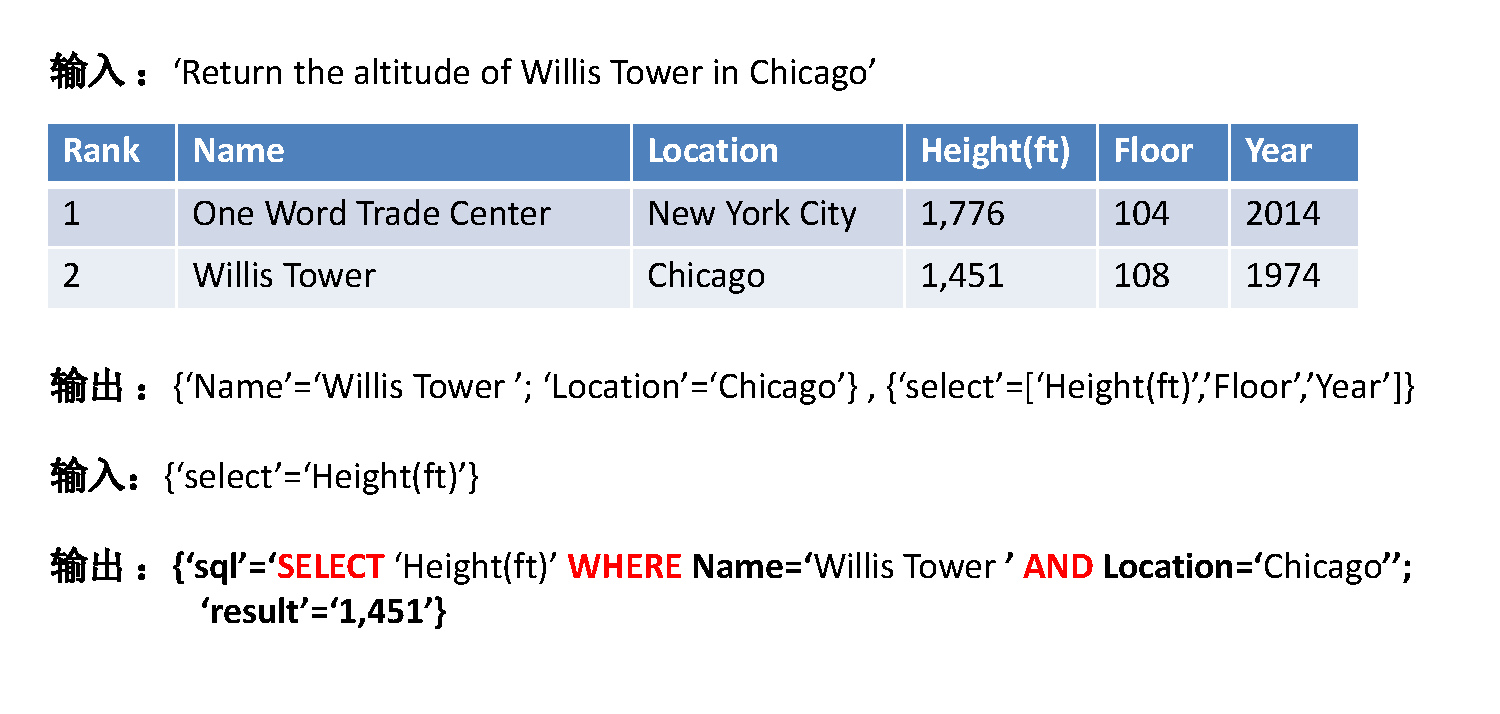
\includegraphics[width=18cm]{example/nli.pdf}
  \bicaption[基于映射的INL2SQL生成示例]
    {基于映射的INL2SQL生成示例}
    {An Example Of Interactive Nature Language To SQL Query Statement With Map}
  \label{fig:NLI}
\end{figure}



图\ref{fig:NLI}中给出了基于映射的INL2SQL生成中的典型的例子。
用户首先输入自然语言查询语句“Return the altitude of Willis Tower in Chicago”以及给出对应的数据库表模式(包含表、列名等)。
系统判断出两个有效过滤条件即‘Name’=‘Willis Tower ’和‘Location’=‘Chicago’但不确认聚合函数是否为‘SELECT’及其对象是否为‘Height(ft)’。系统返回一个包含{‘Name’=‘Willis Tower ’; ‘Location’=‘Chicago’}和{‘select’=[‘Height(ft)’,’Floor’,’Year’]}的交互项。
其中{‘Name’=‘Willis Tower ’; ‘Location’=‘Chicago’}为json格式并表示为已经确认的信息,{‘select’=[‘Height(ft)’,’Floor’,’Year’]}为json格式表示需要用户在‘Height(ft)’,’Floor’,’Year’中做出选择。
用户接受到交互信息后进行选择并发送包含{‘select’=‘Height(ft)’}的json数据。
最后,系统在多轮交互并确认输出有效后将对应的SQL查询语句‘SELECT ‘Height(ft)’ WHERE Name=‘Willis Tower’ AND Location=‘Chicago’及执行结果‘1,451’输出。

% 自然语言理解存在许多难题,如歧义、语序,或者存在复杂的依赖结构等等,要完全基于自然语言理解来进行SQL生成是很困难的,效果可能会不尽如人意。
% 所以,受到人机交互思想的启发,本文将使用自然语言理解与人机交互相结合的方式,来进行从自然语言到目标SQL语句的转化。
% 对于自然语言意图,先对自然语言进行初步解析和理解,并在其中插入人机交互机制,让用户来引导生成的过程,指导自然语言理解,纠正机器理解过程中出现的错误、歧义、含糊不清的问题,从而提升整体的准确性。



\section{相关技术}
% \subsection{相关技术1}
% \subsection{相关技术2}
在软件产品的开发与使用过程中,非专家用户常常会在指定的关系型数据库上使用关键字搜索[!!引用!!]来进行实时的查询。
所以近段时间以来,有很多的研究人员对关键字搜索领域进行研究[!!引用!!]。
关键字搜索的目的不是通过输入的关键字的集合来找到与这些关键字相关联的数据,而是通过这些关键字来推测并解析出其背后想要表达的查询意图及对应的自然语言。
在这些研究中,有的方法通过聚合函数[!!引用!!]、布尔运算符[!!引用!!]、查询语句片段[!!引用!!]等方式对关键字进行拓展。
现在看来,这些研究内容是解决自然语言查询这一挑战的奠基者。
本章所提出的解决方案能够支持更加丰富的查询,使得用户可以使用语义更加复杂的语句进行查询。

数据库的自然语言接口(NLIDB)已经被研究人员研究了很长的时间[!!引用!!]。
早期的NLIDB需要依靠为每个数据库单独定制的手工语法来进行查询,这些手工语法的拓展性很差,很难在其他数据库中进行使用。
相比之下,本章所提出的解决方案以生成SQL查询语句作为目的,具有很好的通用性,可以被移植到其他的数据库上使用。
 
如[!!引用!!]所指出,NLIDB在使用上最大的问题在于其所依赖的信息很有限,正常的自然语言往往是没有一个固定的格式和语义。
这也就导致了NLIDB无法准确地推断用户输入的查询意图。
为了解决可靠性的问题,[!!引用!!]等人采用了PRECISE方法,将输入的自然语言查询划分为语义更加容易被解析的查询片段,并将这些查询片段更为精确地转换为SQL查询语句。
但是,PRECISE无法处理那些语义不确切或者难以处理的自然语言查询。
相比而言,本章提出的解决方案通过与用户的多轮交互,可以较好地解决语义不明确的问题。

也有很多文献[!!引用!!]提出过交互式NLIDB的想法,早期交互式NLIDB[!!引用!!]主要目标在于从查询生成对应的结果。
而NaLIX[!!引用!!]则更进一步,当用户的查询超出模型的语义理解能力的范围之外时会把相应的重构查询的建议返回给用户,这种策略会大大减少用户在使用时对其查询进行重构的负担。
然而,NaLIX对输入的查询超过模型的语义理解能力的处理方式不太正确。
而在本章提出的解决方案中,对于给定的自然语言查询语句,我们会与用户多轮交互并向用户解释我们解析的过程以及生成SQL的过程,从而对查询进行重构,解决起义问题。
所以,在与用户的多轮反馈与交互下,用户在使用我们的系统时可以放心地输入较为复杂的查询,其生成的SQL查询语句可以包含多级聚合操作、嵌套以及各种类型的连接操作等。

总而言之,本章提出的解决方案具有较好的通用性,能够解决语义不明确的问题,可以通过与用户的多轮交互向用户解释我们解析的过程以及生成SQL的过程从而对查询进行重构。

\section{解决方案}
\begin{figure}[!htp]
    \centering
    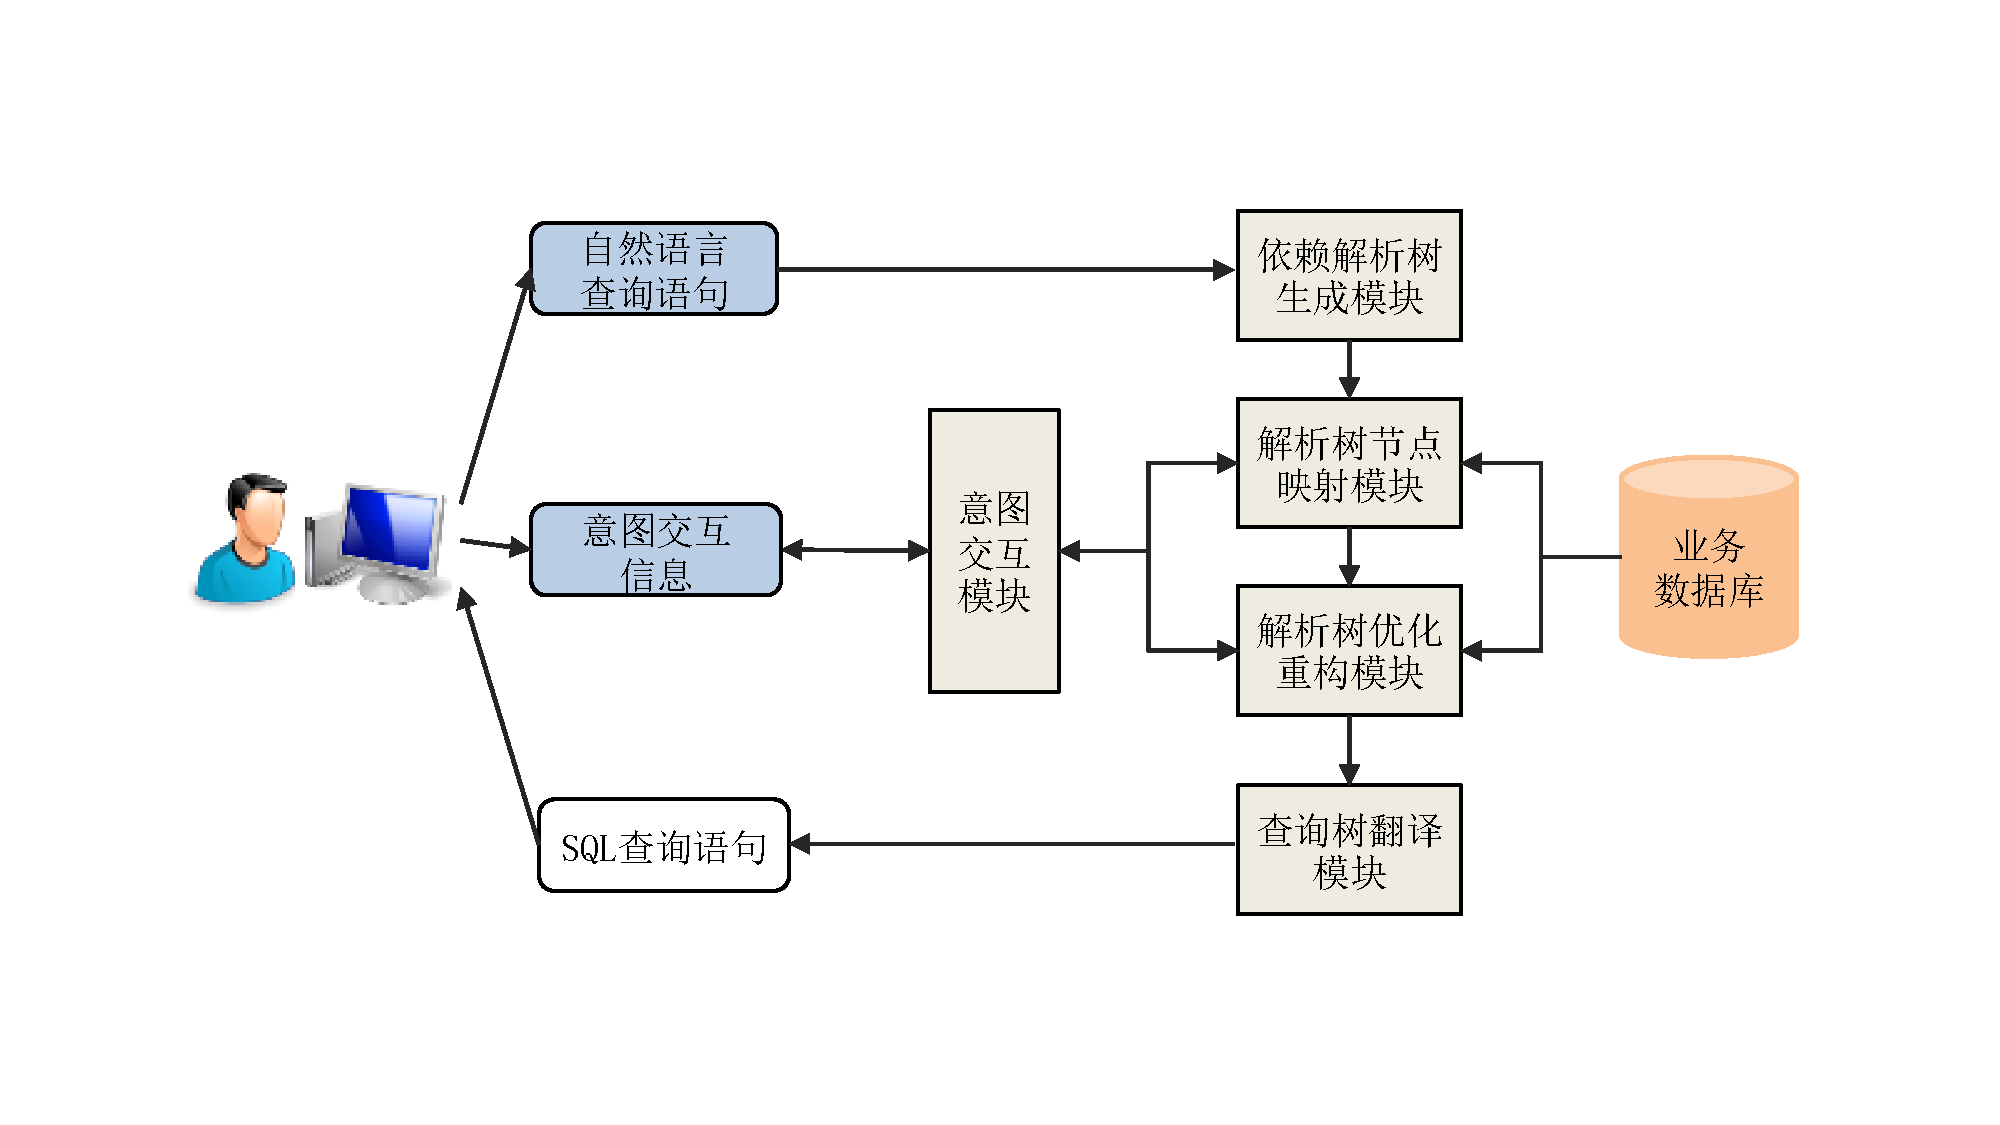
\includegraphics[width=15cm]{example/NLIapproach.pdf}
    \bicaption[基于映射的INL2SQL生成的总体方案]
      {基于映射的INL2SQL生成的总体方案}
      {An Overview Of Interactive Nature Language To SQL Query Statement With Map}
    \label{fig:NLIapproach}
  \end{figure}
图\ref{fig:NLIapproach}是本文从自然语言生成SQL语句模型的总体方案,它包含依赖解析树生成、解析树节点映射、解析树优化重构、查询树翻译、交互式对话器、用户接口六个模块:
\begin{enumerate}
    \item 用户接口:用户与系统进行交互的接口,包括输入自然语言、返回SQL语句、解析过程中的交互等等。
    \item 交互式对话器:管理解析过程与用户的交互,在适当的时候与用户进行交互,让用户对解析过程进行指导。
    \item 依赖解析树生成:将用户输入的,以自然语言表示的查询意图,应用自然语言理解技术,转化为依赖解析树,即将词语进行词性标注,以及识别出词语之间的关系,并将其组织成一个树状结构。详见\ref{nli:yljxssc}节。
    \item 解析树节点映射:根据解析树节点对应的词语和数据库元数据、数据、SQL语法等信息,将解析树节点映射为SQL语法组件。
在这个过程中,如果节点的映射有多个候选答案,交互式对话器会发起与用户的交互,将多个候选映射展示给用户,让用户来进行选择。详见\ref{nli:jxsjdys}节。
    \item 解析树优化重构:节点映射完毕后,解析树节点经过系统匹配和用户指导后,得到了比较准确的结果,但解析树的结构仍是最初由依赖解析树生成得到的结构,这一原始结构的准确度并不高,受限于自然语言的复杂性和省略性,可能会有错误关系、缺失关系、缺失节点等等。
为了使解析树能得到比较准确的结构,将设计算法和规则,修正错误关系,补全缺失节点和缺失关系,得到较为准确的解析树,称为查询树。详见\ref{nli:jxsyhcg}节。
    \item 查询树翻译:解析树的结构已经符合SQL语法,节点映射结果也对应于真实的SQL语法、数据库schema或数据,可以很自然地将树状结构的翻译为SQL语句,最后将SQL语句通过用户接口返回给用户。详见\ref{nli:cxsfy}节。
\end{enumerate}

% 1)	用户接口:用户与系统进行交互的接口,包括输入自然语言、返回SQL语句、解析过程中的交互等等。
% 2)	交互式对话器:管理解析过程与用户的交互,在适当的时候与用户进行交互,让用户对解析过程进行指导。
% 3)	依赖解析树生成:将用户输入的,以自然语言表示的查询意图,应用自然语言理解技术,转化为依赖解析树,即将词语进行词性标注,以及识别出词语之间的关系,并将其组织成一个树状结构。详见3.2节。
% 4)	解析树节点映射:根据解析树节点对应的词语和数据库元数据、数据、SQL语法等信息,将解析树节点映射为SQL语法组件。在这个过程中,如果节点的映射有多个候选答案,交互式对话器会发起与用户的交互,将多个候选映射展示给用户,让用户来进行选择。详见3.3节。
% 5)	解析树优化重构:节点映射完毕后,解析树节点经过系统匹配和用户指导后,得到了比较准确的结果,但解析树的结构仍是最初由依赖解析树生成得到的结构,这一原始结构的准确度并不高,受限于自然语言的复杂性和省略性,可能会有错误关系、缺失关系、缺失节点等等。为了使解析树能得到比较准确的结构,将设计算法和规则,修正错误关系,补全缺失节点和缺失关系,得到较为准确的解析树,称为查询树。详见3.4节。
% 6)	查询树翻译:解析树的结构已经符合SQL语法,节点映射结果也对应于真实的SQL语法、数据库schema或数据,可以很自然地将树状结构的翻译为SQL语句,最后将SQL语句通过用户接口返回给用户。详见3.5节。

接下来,将详细阐述依赖解析树模块、解析树节点映射模块、解析树优化重构模块、查询树翻译器的设计思路和实现细节。

\subsection{依赖解析树生成}
\label{nli:yljxssc}

本模块将用户输入的自然语言查询意图解析为解析树,包含各词语的词性标注、关系提取等等信息。
在具体实现过程中,这一模块基于StanfordCoreNLP[!!!!!!!!!!!此处引用]实现。
StanfordCoreNLP是斯坦福大学推出的自然语言处理工具集,支持多种语言,还提供了C++、Python、Java等多种程序语言的编程接口,提供依赖解析、命名实体识别、词性标注、情感分析、机器翻译等多种功能。
本模块调用该工具,将自然语言解析为依赖解析树。

\subsection{解析树节点映射}
\label{nli:jxsjdys}
本模块将依赖解析树的节点对应的词语,映射到SQL组件上。解析树节点的类型定义如表\ref{nli:jxsjddlx}所示。

% 这一节给出的是一些表格的例子,如表\ref{nli:jxsjddlx}所示。

\begin{table}[!hpb]
  \centering
  \bicaption[解析树节点的类型]
    {解析树节点的类型}
    {Different Types of Nodes}
  \label{nli:jxsjddlx}
  \begin{tabular}{@{}llr@{}} \toprule
    % \multicolumn{2}{c}{Item} \\ \cmidrule(r){1-2}
    节点类型 & 对应的SQL组件\\\midrule
    选择节点(SN) & SELECT\\
    操作符节点(ON) & 一个操作符,如等于(“=”)、小于(“<”)\\
    聚合函数节点(FN) & 一个聚合函数,如AVG、MAX\\
    名字节点(NN) & 业务数据库中的一个数据表的名字,或数据表的一个字段的名字\\
    值节点(VN) & 业务数据库中某字段的一个值\\
    度量节点(QN) & ALL,ANY,EACH\\
    逻辑节点(LN) & AND,OR,NOT\\\bottomrule

    % Animal & Description & Price (\$)\\ \midrule
    % Gnat & per gram & 13.65 \\
    % & each & 0.01 \\
    % Gnu & stuffed & 92.50 \\
    % Emu & stuffed & 33.33 \\
    % Armadillo & frozen & 8.99 \\ \bottomrule
  \end{tabular}
\end{table}
% \footnotetext[1]{这个例子来自\href{http://www.ctan.org/tex-archive/macros/latex/contrib/booktabs/booktabs.pdf}{《Publication quality tables in LATEX》}(booktabs宏包的文档)。这也是一个在表格中使用脚注的例子,请留意与threeparttable实现的效果有何不同。}


其中名字节点和值节点是与当前应用的业务数据库有关,其余五种节点都与业务数据库无关,仅与SQL语法规则相关。
所以,本系统建立了一个五种与业务数据库无关的节点类型与自然语言单词的词典映射。映射过程的实现如下:
对每一个解析树节点对应的单词$n$,分别计算其与业务数据库元数据、存储数据、词典映射中词语v的相似度$Sim_{wup}(n,v)$,$Sim_{gram}(n,v)$的定义如公式\ref{nli:eq1}所示:

%   \begin{equation}
%     \label{eq:res}
%     \ointop_{\gamma}f(z)\,\mathrm{d}z = 2\uppi\mathbf{i}\sum^n_{k=1}\mathrm{I}(\gamma,a_k)\mathrm{Res}(f,a_k)
%   \end{equation}
  \begin{equation}
    \label{nli:eq1}
    % Sim \left ( n ,\right v) = \max\left ( Sim_{wup}\left ( n ,\right v) ,\right Sim_{gram}\left ( n ,\right v))
    Sim(n,v) = \max(Sim_{wup}(n,v),Sim_{gram}(n,v))
\end{equation}

其中$Sim_{wup}(n,v)$为$n$和$v$的WUP相似度[!!引用!!],$Sim_{gram}(n,v)$为$n$和$v$的q-gram的Jaccard相似度的平方根[!!引用!!]。
经公式计算,可以得到节点单词$n$与所有SQL组件的相似度;
对相似度进行排序,可以得到前五相似的SQL组件,如果前五相似的SQL组件的相似度$Sim(n,v)$的值差别较大,则直接以相似度最高的SQL组件作为当前单词n的映射,并赋予该组件对应的节点类型;
若前五相似的SQL组件的相似度差别较小,则视作歧义,将候选的SQL组件返回给用户,让用户来进行选择,最后用户选择的结果会作为当前节点的映射。 

\subsection{解析树优化重构}
\label{nli:jxsyhcg}

节点映射完成后,需要对解析树的结构进行重构,保证解析树的结构能有较高的准确性。
由于解析树可能会存在关系解析错误和节点关系缺失,所以这一模块对于解析树的优化重构会分为两个步骤进行,分别为结构调整和隐藏节点插入。

\subsubsection{结构调整}

在进行结构调整之前,首先定义什么样的树结构是好的、合法的。
我们从两个角度来考虑这个问题:第一点是树结构与经依赖解析器解析后的原始结构的差别有多大;
第二点是树结构是否符合SQL的语法,这一点的评估可以根据表\ref{nli:hfjxsjggz}的定义来确定[!!yinyong!!]。

\begin{table}[!hpb]
    \centering
    \bicaption[合法解析树结构规则]
      {合法解析树结构规则}
      {Grammar of Valid Parse Trees}
    \label{nli:hfjxsjggz}
    \begin{tabular}{@{}llr@{}} \toprule
      % \multicolumn{2}{c}{Item} \\ \cmidrule(r){1-2}
      1  & 	Q -> ( SClause ) ( ComplexCondition ) *\\
      2  & 	SClause -> SELECT + GNP\\
      3  & 	ComplexCondition -> ON + ( leftSubtree * rightSubtree )\\
      4  & 	leftSubtree -> GNP\\
      5  & 	rightSubtree -> GNP | VN | MIN | MAX\\
      6  & 	GNP -> ( FN + GNP ) | NP\\
      7  & 	NP -> NN + ( NN ) * ( Condition ) *\\
      8  & 	condition -> VN | ( ON + VN )\\\bottomrule
    \end{tabular}
  \end{table}

表\ref{nli:hfjxsjggz}根据SQL语句的语法,结合了树状结构,定义了能合理的转化为SQL语句的语法树应该满足什么样的规则,这样的语法树我们称之为查询树。
在表\ref{nli:hfjxsjggz}中,“ + ”代表父子节点的关系,“ * ”代表兄弟节点的关系,上标“ * ”代表可重复出现的兄弟节点,“ | ”代表“或者关系”,表示当前节点可能存在的情况。
% 这是写在算法\ref{algo:sum_100}前面的一段话,在生成的文件里它会出现在算法\ref{algo:sum_100}前面。
\begin{algorithm}
    % \begin{algorithm}[H] % 强制定位
    \caption{解析树结构调整算法}
    \label{nli:jxsjgtzsf}
    \begin{algorithmic}[1] %每行显示行号
    \Ensure 结构调整之后的解析树结果集 % 输出
    % \State $sum \gets 0$
    % \For{$i = 0 \to 100$}
    %     \State $sum \gets sum + i$
    %   \EndFor
    \State $results \gets empty\_set()$
    \State $priorityQueue \gets empty\_priority\_queue()$
    \State $priorityQueue \gets priorityQueue + parseTree$
    % priorityQueue.push(parseTree)
    \State $hash\_table \gets empty\_set()$
    \State $hash\_table \gets hash\_table +hash(parseTree)$
    % hash\_table.add(hash(parseTree))
    \While{$priorityQueue != empty\_priority\_queue()$}
        \State $tree \gets priorityQueue.pop()$
        \State $treeList \gets adjust(tree)$
        \For{$adjustTree in treeList $}
        \If{$hash(adjustTree) not in hash\_table$ \textbf{and} $adjustTree.edit < t$}
            \State $adjustTree.edit \gets tree.edit + 1$
            \State $hash\_table \gets hash\_table + hash(adjustTree)$
            % hash\_table.add(hash(adjustTree))
            \If{$evaluate(adjustTree) >= evaluate(tree)$}
                \State $priorityQueue.add(tree’)$
            \EndIf
            \If{adjustTree is valid}
                \State $results.add(adjustTree)$
            \EndIf
        \EndIf
        \EndFor
    \EndWhile
    \State $results \gets rank(results)$
    \State \Return$results$
    \end{algorithmic}
    \end{algorithm}
算法\ref{nli:jxsjgtzsf}展示了结构调整的算法,算法的基本思想是,建立一个优先级队列,对于当前的解析树,调用adjust()函数(第8行),通过一次移动子树操作,生成在这一次操作后所有可能的结构;
然后记录当前树的哈希值(第12行),防止之后出现重复的树结构;
若当前树结构没有出现过(第10行),且edit值小于一个阈值,则对此树进行下一步操作;
由于移动了一次子树,返回的树的edit属性加一(第11行),这一属性将用来评估生成的树结构与原始结构的差异;
调用evaluate()函数,记录当前结构有多少节点不满足表\ref{nli:hfjxsjggz}设定的规则,不满足规则的节点数将用来评估树结构在语法上的合法性;
综合这两方面评估标准,为树打分,如果分数比之前的树结构要高,则加入优先级队列;
若该树完全符合语法规则,则视为一颗查询树,加入result集合;
之后对优先级队列内的树结构重复以上操作,直到优先级队列为空;最后根据评估分数对result集合排序,将结果返回。

结构调整之后的解析树结果集,将会通过交互式对话器,与用户进行交互,因为结果集中的解析树虽然都符合SQL语法规则,但仍有可能存在与用户意图不同的情况,如SELECT子句中的名字节点和WHERE子句中的名字节点,位置可能会互换,虽然仍然符合SQL语法规则,但与原始查询意图已经有比较大的差别了。
所以,在这里需要再一次应用人机交互机制,让用户来选择结果集中与自己的查询意图比较相似的解析树。交互完成后,筛选出的结果集,会进入下一步——隐藏节点插入。

\subsubsection{隐藏节点插入}

结构调整完成后,对经过排序和用户交互筛选后的结果集合,进行隐藏节点插入。
在给出隐藏节点插入的方法之前,先给出需要用到的概念定义,即“核心节点”。
核心节点指的是在节点类型为leftSubtree和rightSubtree的情况下(表\ref{nli:hfjxsjggz}),leftSubtree(rightSubtree)的所有子节点中,高度最高的名称节点被称为核心节点。

经过研究,需要进行隐藏节点插入的情况有以下几种:
\begin{enumerate}
    \item 左子树(leftSubtree)与右子树(rightSubtree)的核心节点对应了不同的SQL组件,即认为右子树真正的核心节点在自然语言表达时被省略了[14];
    这是十分常见的现象,因为人在进行自然语言表达时,对两个值进行比较时,会很自然的省略掉后者的一部分,如“Ihavemorebooksthanyours”这句话,就将最后的“yourbooks”给省略成了“yours”;
    \item 左右子树的约束条件应该一致,如果不一致,则认为右子树一部分约束条件被省略了,如“returnauthorswhosepaperspublishedin2018morethanJack’s”这句话,过滤条件的左子树有“in2018”这一约束,而右子树在解析之后没有这一约束,事实上右子树的这一约束被隐藏了,需要作为隐藏节点插入进去;
    \item 某些函数会被省略,如聚合函数“COUNT”,在自然语言表达中经常会被省略,如“Ihavemorebooksthanyours”这句话,“thenumberof”就被省略了。在树结构中,如果过滤条件的操作符为“more”、“less”等词语,而左右子树的核心节点对应的是非数字类型的SQL组件,那么就认为“COUNT”被省略了,需要作为隐藏节点插入解析树。
\end{enumerate}
% 1)	左子树(leftSubtree)与右子树(rightSubtree)的核心节点对应了不同的SQL组件,即认为右子树真正的核心节点在自然语言表达时被省略了[14];这是十分常见的现象,因为人在进行自然语言表达时,对两个值进行比较时,会很自然的省略掉后者的一部分,如“Ihavemorebooksthanyours”这句话,就将最后的“yourbooks”给省略成了“yours”;
% 2)	左右子树的约束条件应该一致,如果不一致,则认为右子树一部分约束条件被省略了,如“returnauthorswhosepaperspublishedin2018morethanJack’s”这句话,过滤条件的左子树有“in2018”这一约束,而右子树在解析之后没有这一约束,事实上右子树的这一约束被隐藏了,需要作为隐藏节点插入进去;
% 3)	某些函数会被省略,如聚合函数“COUNT”,在自然语言表达中经常会被省略,如“Ihavemorebooksthanyours”这句话,“thenumberof”就被省略了。在树结构中,如果过滤条件的操作符为“more”、“less”等词语,而左右子树的核心节点对应的是非数字类型的SQL组件,那么就认为“COUNT”被省略了,需要作为隐藏节点插入解析树。

进行隐藏节点插入之后,查询树的结构就比较完整了,将会输入下一模块进行翻译。

\subsection{查询树翻译}
\label{nli:cxsfy}
这一阶段的查询树已经在节点映射、树结构、完整性方面都比较可信、合法了,翻译步骤如下:
\begin{enumerate}
    \item 根据表\ref{nli:hfjxsjggz}中的树结构,在SClause子树下的结构为SELECT子句,读取SClause下的名称节点,根据对应的SQL组件(如果SQL组件对应某数据表,该数据表会预定义一个核心字段,如用户的名字、城市的名称,该数据表的核心字段将作为结果返回),填充入SELECT子句,并记录SQL组件对应的数据表,以备FROM子句的生成。
    \item 在ComplexCondition子树下的结构为WHERE子句,分别读取左子树和右子树核心节点对应的SQL组件,记录下SQL组件对应的数据表,并查看左右子树中所有的节点,根据其节点类型,将其翻译为对应的SQL组件,并应用于核心节点;左右子树解析完后,以操作符连接左右子树,将其填充入WHERE子句。
    \item 根据之前记录的相关数据表,生成SQL语句的FROM子句。
    \item 将三部分按照语法连接起来,作为合法的SQL语句返回给用户。
\end{enumerate}

\section{实验与分析}

\subsection{数据集}
本次实验所使用的业务数据库为MySQL的样例数据库Classicmodels,图3-2为Classicmodels数据库的数据库模式图
\begin{figure}[!htp]
    \centering
    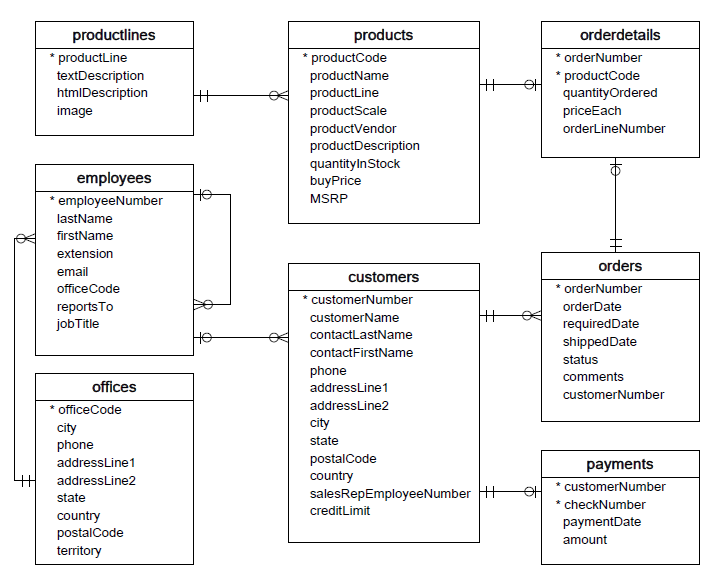
\includegraphics[width=15cm]{example/classicmodel.png}
    \bicaption[Classicmodels数据库的数据库模式图]
      {Classicmodels数据库的数据库模式图}
      {Database Schema of Classicmodels Database}
    \label{fig:NLIclassicmodel}
  \end{figure}

实验所使用的自然语言查询数据集由作者根据Classicmodels数据库的模式建立,根据查询意图的复杂度,分为简单、中等、困难三类。每种类别,提出了20条自然语言查询,共计60条,用来测试模型的准确性。
表\ref{nli:zryycxsl}给出了三种类别的自然语言查询示例。

\begin{table}[!hpb]
    \centering
    \bicaption[自然语言查询实例]
      {自然语言查询实例}
      {Instances Of Natural Qanguage Query}
    \label{nli:zryycxsl}
    \begin{tabular}{cc} \toprule
      % \multicolumn{2}{c}{Item} \\ \cmidrule(r){1-2}
      查询语句复杂度 & 示例\\\midrule
      简单 & return all the custormers\\
      中等 & return all the offices in London\\
      困难 & return the city of office that has an employee named Diane\\
      \bottomrule
    \end{tabular}
  \end{table}

\subsection{实验结果}

首先将所有自然语言查询语句,输入系统,经过各组件的处理,得到系统生成的SQL语句,再判断其是否正确表达了自然语言查询语句的意图。
实验结果如表\ref{nli:mxscsyjdzqx}所示。

\begin{table}[!hpb]
    \centering
    \bicaption[模型生成SQL语句的准确性]
      {模型生成SQL语句的准确性}
      {The Accuracy Of Generating SQL Statements}
    \label{nli:mxscsyjdzqx}
    \begin{tabular}{cc} \toprule
      % \multicolumn{2}{c}{Item} \\ \cmidrule(r){1-2}
      查询语句复杂度 & 准确率\\\midrule
      简单 & 100\%\\
      中等 & 80\%\\
      困难 & 35\%\\
      \bottomrule
    \end{tabular}
\end{table}

实验还检验了在没有用户交互指定节点映射、选择合适树结构的情况下,模型生成SQL语句的准确性,如表\ref{nli:mxzwjhqkxscsyjdzqx}所示;
由于没有选择合适树结构,导致解析树结构调整之后有多个候选结果,最后返回结果也会有多个,故只要返回结果中包含正确SQL语句,就视做正确生成:

\begin{table}[!hpb]
  \centering
  \bicaption[模型在无交互情况下生成SQL语句的准确性]
    {模型在无交互情况下生成SQL语句的准确性}
    {The Accuracy Of Generating SQL Statements Without Interaction}
  \label{nli:mxzwjhqkxscsyjdzqx}
  \begin{tabular}{cc} \toprule
    % \multicolumn{2}{c}{Item} \\ \cmidrule(r){1-2}
    查询语句复杂度 & 准确率\\\midrule
    简单 & 65\%\\
    中等 & 50\%\\
    困难 & 15\%\\
    \bottomrule
  \end{tabular}
\end{table}

\subsection{实验分析}
\begin{enumerate}
    \item 经过两次实验,分别检验完整模型和无交互机制模型生成SQL语句的准确性。可以看出,交互机制对于模型的准确性有很大的提升;而加入了交互机制后,模型可以比较准确的处理简单和中等复杂度的查询意图,即便是复杂度较高的查询意图,本文提出的模型仍然可以正确生成一部分困难复杂度的SQL语句。在实验过程中,经常出现节点歧义需要映射,如“price”一词可以映射到“products”表中的“buyPrice”,也有可能映射到“orderdetails”表中的“priceEach”。那么对于测试语句“return order details whose price is higher than 50”,如果没有交互机制,对于“price”这个节点的映射就会优先映射到“products”中的“buyPrice”,而实际上应该映射到“orderdetails”表中的“priceEach”。可以看出,交互机制在节点映射这一部分准确率的提升,大大影响了整体模型的准确率。
    \item	在作者构造的自然语句查询意图数据集中,简单复杂度的查询意图大体上是返回某数据表中某一字段,中等复杂度的查询意图会添加一些聚合函数和简单过滤条件,困难复杂度的意图会增加更多的聚合函数和跨表查询,总体上来说结构都比较简单。在表3-5所示的结果中,困难复杂度意图的错误生成情况,一部分来源于查询意图对应的SQL语句需要子查询,如“return the customer who has the most orders”。目前的模型还不能很好的处理这一种情况,在解析树语法和翻译过程中都还没考虑子查询的情况,这可能是接下来需要进一步进行的工作,即提升模型的处理能力,使其能处理更复杂的查询意图。
    \item	目前模型基于相似度的节点映射机制仍然有不足之处,如“return the mobile number of custormer whose name is Australian Gift Network”这一查询意图,对于顾客名称“Australian Gift Network”,系统会将其映射为三个不同的节点,导致生成出错。尽管模型对于数据库模式中的一些连接词或短语,如“thenumberof”、“customername”,进行了特殊处理,但对于上文所示的这些特殊短语或词语,目前没有较好的方法来进行处理。
    \item	本文自行建立了一个解析树节点类型与自然语言单词的映射词典(表\ref{nli:jxsjddlx}),能处理一些常见的单词与SQL语法的对应关系,如“return”、“in”、“have”、“thenumberof”,但映射关系仍然不足,所以本实验所使用的测试查询意图都需要使用这些比较固定的词语来构建。事实上,自然语言的表达非常多样,如果要增加模型的处理能力,扩充这个映射词典也是非常必要的。
    \item	尽管人机交互机制对于节点映射的准确率有较大提升,但根据观察,立足于目前数据量较小、数据库模式简单的前提下,这一机制能保证映射相似度排名前五的SQL组件包含正确的映射关系;但随着数据库数据量的增加、数据库模式的复杂化,目前节点映射的相似度计算机制,可能无法确保正确的SQL组件能有较高的相似度。
\end{enumerate}

\section{本章小结}
本章提出了交互式自然语言接口生成SQL语句模型的设计和具体实现,基本思想是结合自然语言解析技术,使用人机交互的方式指导解析过程,减轻自然语言解析的歧义问题和错误情况,相比于纯自然语言解析技术,大大提升了准确性。
本章针对自然语言生成SQL模型的准确性进行了实验,实验数据库为MySQL样例数据库classicmodels,测试用自然语言查询意图为作者自行根据实验数据库建立,分别包含简单、中等、困难三种复杂度的查询意图。以此为测试数据集,对完整模型和无交互机制的模型进行了实验,并给出了实验结果。结果发现,完整模型能较好的处理简单和中等复杂度的查询意图,一定程度上能处理困难复杂度的查询意图,而且经过与无交互机制的模型进行对比,发现交互机制对于模型准确度的提升十分显著。但对实验结果进行细致分析,也发现模型存在处理能力仍然不足、无法处理子查询、自然语言意图形式比较固定、无法处理特殊词组等问题,需要进一步进行提升和改进。





%# -*- coding: utf-8-unix -*-
% !TEX program = xelatex
% !TEX root = ../thesis.tex
% !TEX encoding = UTF-8 Unicode
%%==================================================
%% chapter02.tex for SJTU Master Thesis
%% based on CASthesis
%% modified by wei.jianwen@gmail.com
%% Encoding: UTF-8
%%==================================================

\chapter{基于深度强化学习的NL2SQL生成}
\label{chap:enl2sql}

\section{研究问题}

随着计算机技术的快速发展与应用,关系型数据库被广泛应用于教育、医疗、商业等领域。
作为信息存储的载体,越来越多的软件开发和业务人员正频繁使用SQL查询语句来读取关系型数据库中的数据。
SQL语句用法多样且功能强大,但对于一个没有技术背景的使用者来说却是一场噩梦。
即便是一名专业的软件人员,在面对数据库中众多的实体以及每个实体都有自己独特的含义时,想要把SQL语句写正确也不是一件容易的事情。
因此,学术界和工业界一直都在思考如何更快更好地使用SQL语句来读取数据,其中最理想和最直接的方式便是直接让使用者使用自然语言从数据库中获取所需信息。

实现这个目标的关键在于如何去理解自然语言语句的意图并讲其映射到SQL语句上,简称为NL2SQL(Nature Language To SQL Statement),即自然语言生成SQL查询语句任务。
在NL2SQL任务中,一个典型的例子如图\ref{fig:nl2sqlexample}给出。

\begin{figure}[!htp]
    \centering
    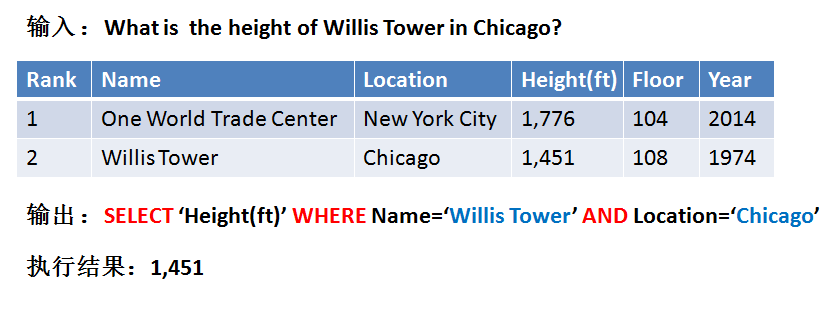
\includegraphics[width=15cm]{example/nl2sql.png}
    \bicaption[这里将出现在插图索引中]
      {NL2SQL的一个典型示例}
      {English caption}
    \label{fig:nl2sqlexample}
  \end{figure}

图\ref{fig:nl2sqlexample}为WikiSQL数据集[!!引用!!]中的一个样例。
WikiSQL数据集是纯自然语言生成SQL查询语句的第一个数据集。
其中包含80654组自然语言问句及其对应的SQL查询语句,涵盖24241张从Wikipedia中获取的数据表。
从图中可以看到,NL2SQL任务的输入实际包括两部分:自然语言问题以及一个简单的数据表schema(schema代表数据表及表中的列)。

WikiSQL数据集中SQL查询语句具有一定的约束条件,必须符合如下模板:

\begin{table}[!hpb]
    \centering
    \bicaption[指向一个表格的表目录索引]
      {SQL查询语句模板}
      {A Table}
    \label{nli:sqlmb}
    \begin{tabular}{@{}llr@{}} \toprule
      % \multicolumn{2}{c}{Item} \\ \cmidrule(r){1-2}
    %   节点类型 & 对应的SQL组件\\\midrule
    \emph{SELECT   agg   selcol   WHERE   col   op   val   (AND   col   op   val)*}\\\bottomrule
  
      % Animal & Description & Price (\$)\\ \midrule
      % Gnat & per gram & 13.65 \\
      % & each & 0.01 \\
      % Gnu & stuffed & 92.50 \\
      % Emu & stuffed & 33.33 \\
      % Armadillo & frozen & 8.99 \\ \bottomrule
    \end{tabular}
  \end{table}

  在\ref{nli:sqlmb}中,\emph{selcol}代表表中的列名,\emph{agg}代表聚合操作(例如:COUNT,SUM或空),
  \emph{WHERE}后面为由一系列过滤调教构成的子句,每个\emph{op}代表一个过滤操作(例如:“=”),\emph{val}代表出现在自然语言问句中的过滤值。
  值得注意的是,尽管模板中的过滤条件服从标准的线性顺序,但由于存在\emph{AND}符号,所以过滤条件的先后顺序是无关紧要的。

  在后文中,我们声明如下一些表示:总输入表示为$x$,其包含由单词$w_{i}$组成的自然语言问题$w$以及由列名$c_{j}$组成的单张表的schema $c$(其中,列名$c_{j}$可由单个或多个单词组成)。
  最后,我们的模型需要生成一条可执行的SQL查询语句$y$作为输出。

\section{相关技术}
\subsection{NL2SQL研究现状}
\subsection{深度学习}
\subsection{强化学习}
\subsection{语义解析}
\section{解决方案}

\subsection{增强解析器模型}
\label{enl2sql:zqjxqmx}
针对每个输入$x$来生成结构化的输出$y$的过程可以被分解成为一系列的语义解析决策的过程。
所以,增强解析器模型的基本思路为:解析器从初始状态启动并不断根据学习的策略采取不同的操作。
每个动作(action)都会将解析器从一个状态(state)转移为另一个状态,知道解析器到达它的最终状态并停止。
在解析器的最终状态下,我们可以获取一个完整的输出$y$。
我们采取一种概率的方法来对整个的策略(policy)建模。
它可以对由输入$x$产生的有效的动作(action)的集合以及解码器产生的历史行为进行概率分布进行预测。
所以,整个增量语义解析器的训练目标就转换为了如何优化一个参数化的策略的问题。

% , 其中$\theta$为模型参数。
\begin{equation}
    \label{enl2sql:eq1}
    % Sim \left ( n ,\right v) = \max\left ( Sim_{wup}\left ( n ,\right v) ,\right Sim_{gram}\left ( n ,\right v))
    % Sim(n,v) = \max(Sim_{wup}(n,v),Sim_{gram}(n,v))
    % P_{\theta}(y|x) = P_{\theta}(\boldsymbol{a}|x),   \theta为模型参数
    P_{\theta}(y|x) = P_{\theta}(\boldsymbol{a}|x),  \qquad \theta\text{为模型参数}
\end{equation}

根据公式\ref{enl2sql:eq1},通过执行动作(action)序列$\boldsymbol{a} = \{a_{1},a_{2},...,a_{k}\}$,解析器将被不断引导并从初始状态转换为包含输出$y$的最终状态。
在此,我们需要假设每个输出$y$有且仅有一个对应的动作序列$\boldsymbol{a}$(详见\ref{enl2sql:ndo}节内容)。
行动序列的概率$P_{\theta}(\boldsymbol{a}|x)$可展开为增量策略概率的乘积(公式\ref{enl2sql:eq2}):

\begin{equation}
    \label{enl2sql:eq2}
    % Sim \left ( n ,\right v) = \max\left ( Sim_{wup}\left ( n ,\right v) ,\right Sim_{gram}\left ( n ,\right v))
    % Sim(n,v) = \max(Sim_{wup}(n,v),Sim_{gram}(n,v))
    P_{\theta}(\boldsymbol{a}|x) = \prod^k_{i=1}P_{\theta}(a_{i}|x,a_{<i}),   \qquad |\boldsymbol{a}| = k
\end{equation}

在推断(inference)期间,我们的模型并非尝试枚举整个输出空间并找到最高的得分$\boldsymbol{a}^{*} = \mathop{\arg\max}_{\boldsymbol{a}} P_{\theta}(\boldsymbol{a}|x)$,
而是在解码器中采用了一种贪心的方法:在每一步都根据策略(policy)来选择得分最高的行动,即$a^{*}_{i} = \mathop{\arg\max}_{a_{i}} P_{\theta}(a_{i}|x,a^{*}_{<i})$。

在后面的几节中,我们将给出解析器状态(state)的定义以及动作(action)清单,还会详细介绍整个基于编码器-解码器神经网络体系结构的增强解析器模型。

% \begin{figure}[!htp]
%   \centering
%   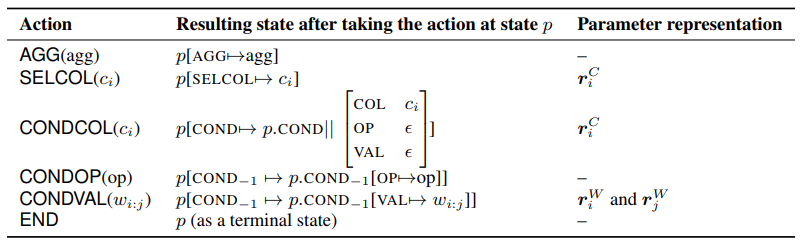
\includegraphics[width=20cm]{example/incsql.png}
%   \bicaption[这里将出现在插图索引中]
%     {中文题图}
%     {English caption}
%   \label{fig:SRR}
% \end{figure}

\subsection{动作序列}
\label{enl2sql:dzxl}

首先,我们给出对应于图\ref{fig:nl2sqlexample}中示例的完全解析之后的结构化表示:
% $\begin{Bmatrix}
%   1 & 2 \\
%   4 & 3 \\
% \end{Bmatrix}$
% \begin{bmatrix}
  
% \end{bmatrix}

$\begin{bmatrix}
  AGG    &  NONE  \\
  SELCOL &  Height(ft) \\
  COND   &   \langle
  % \begin{Bmatrix}
    \begin{bmatrix}
      COL  &  Name \\
      OP   &  =    \\
      VAL  &  “Willis Tower”\\
    \end{bmatrix}
    ,
    \begin{bmatrix}
      COL  &  Location \\
      OP   &  =    \\
      VAL  &  “Chicago”\\
    \end{bmatrix}
    % \end{Bmatrix}
    \rangle
  \end{bmatrix}$

因此,解析器的中间状态就被这样分部表示,其中一些尚未填充的特征值表示为$\epsilon$。
解析器的初始状态$p_{0}$的值为空和空列表,表示为$\begin{bmatrix}
  AGG    &  \epsilon  \\
  SELCOL &  \epsilon \\
  COND   &   \langle \rangle\\
  \end{bmatrix}$。

除此之外,我们还需要定义动作(action)清单。每个动作可以将解析器的状态从一个状态转换为另一个状态,即 $p \rightarrow p_{'}$ 。
我们设$p = \begin{bmatrix}
  AGG    &  agg  \\
  SELCOL &  selcol \\
  COND   &   cond\\
  \end{bmatrix}$,并且在表\ref{enl2sql:dzqd}中给出每个动作执行后的转移状态$p'$。

  \begin{table}[!hpb]
    \centering
    \bicaption[指向一个表格的表目录索引]
      {动作(action)清单}
      {A Table}
    \label{enl2sql:dzqd}
    \begin{tabular}{@{}llr@{}} \toprule
      % \multicolumn{2}{c}{Item} \\ \cmidrule(r){1-2}
      \textbf{动作(action)} & \textbf{由状态}$p$\textbf{执行该动作之后的状态} & \textbf{参数表示}\\\midrule
      % 1  & 	Q -> ( SClause ) ( ComplexCondition ) *\\
      AGG($agg$)  &  $p[AGG \mapsto agg]$  & - \\
      SELCOL($c_i$)  &  $p[SELCOL \mapsto c_i]$  & $r^C_i$ \\
      CONDCOL($c_i$)  &  $p[COND \mapsto p.COND||\begin{bmatrix}
        COL    &  c_i  \\
        OP &  \epsilon \\
        VAL   &   \epsilon\\
        \end{bmatrix}]$  &  $r^C_i$\\
      CONDOP(op)  &  $p[COND_{-1} \mapsto p.COND_{-1}[OP \mapsto op]]$  & -\\
      CONDVAL($w_{i:j}$)  &  $p[COND_{-1} \mapsto p.COND_{-1}[VAL \mapsto w_{i:j}]]$  &  $r^W_i and r^W_j$\\
      END  &  $p$(最终状态)  &  -\\\bottomrule
    \end{tabular}
  \end{table}

需要说明的是,在表\ref{enl2sql:dzqd}中,在解码器中所使用的参数表示将在\ref{enl2sql:decoder}节中进行解释;
$p[AGG \mapsto agg]$表示与状态$p$处于同一状态,不过其特征值$AGG$已经被赋值为$agg$;
$||$表示列表展开;$COND_{-1}$表示在列表中的上一个元素;


值得注意的是,动作$CONDVAL$会从输入问句$w$中选择所需的文字段$w_{i:j}$。
但这样做会导致一个问题,它将产生大量的动作,其数量级为问题长度的二次方。
因此,我们将动作$CONDVAL$分解为两个连续的子动作,一个去选择起始位置$w_i$,另一个则选择终止位置$w_j$。
在动作序列的最后,我们需要增加一个$END$动作来执行解析过程并使解析器进入结束状态。
举例来说,图\ref{fig:nl2sqlexample}中的例子可以看作是如下的一个动作序列:
\begin{enumerate}
  \item $AGG(NONE)$
  \item $SELCOL(c_3)$
  \item $CONDCOL(c_1)$
  \item $CONDOP(=)$
  \item $CONDVAL(w_{5:6})$
  \item $CONDCOL(c_2)$
  \item $CONDOP(=)$
  \item $CONDVAL(w_{8:8})$
\end{enumerate}
% ${AGG(NONE),SELCOL(c_3),CONDCOL(c_1),CONDOP(=),CONDVAL(w_{5:6}),CONDCOL(c_2),CONDOP(=),CONDVAL(w_{8:8})}$

该节中的定义是基于所有有效序列都具有AGG  SELCOL  (CONDCOL  CONDOP  CONDVAL)* END形式的假设之上。
也就保证了我们可以从所有的最终状态中提取出完整的逻辑形式出来。
对于其他不同结构的SQL语句来说,我们还需要重新设计动作的清单以及解析器的状态。


\subsection{编码器}
\label{enl2sql:encoder}

增强解析器模型的架构如图xx所示。

增强解析器模型包含编码器和解码器两个部分,其中编码器的具体步骤如下:
\begin{enumerate}
  \item 对于输入的句子$w$中的每个单词$w_i$,先将其使用词向量进行向量编码(word embedding[!!引用!!])。
  \item 将其送入一个双向的长短期记忆网络(bi-directional Long Short-Term Memory,简称bi-LSTM),其中每个细胞(cell)会有一个隐状态$h^W_i$。
  \item 由于一个列名可能由一个或多个单词构成,我们对每个列名先进行词向量编码并输入一个bi-LSTM中,再使用从bi-LSTM中得到的最终的隐状态作为列名初始表示(initial representation)。
  \item 使用自注意力机制(self-attention[!!引用!!])将该初始表示转换为$h^C_j$。
  \item 在得到基于内容的表示$h^W_i$和$h^C_j$之后,使用cross-serial dot-product attention[!!引用!!]得到$h^C_j$和$h^W_i$的加权平均值并作为单词$w_i$和$c_j$的上下文向量。
  \item 将这两个上下文向量进行拼接并分别送入使用自然语言问题和列名作为输入的bi-LSTM中。这两个LSTM网络的隐状态就是我们所期望的和上下文相关的表达$r^W_i$和$r^C_j$。
\end{enumerate}


\subsection{解码器}
\label{enl2sql:decoder}

在\ref{enl2sql:encoder}节中,我们已经获得了对于单词$w_i$上下文相关的表示$r^W_i$和以及列名$c_j$的上下文相关的表示$r^C_j$。
接下来是解码器部分的设计与细节。

首先,解码器的目标是为了对由输入$x$和历史活动$a_{<i}$构成的概率分布$P_{\theta}(a|x,a_{<i})$进行建模。其主要包括以下两点挑战:
\begin{enumerate}
  \item 活动(action)的不确定性:所有活动均需要取决于输入以及当前解析器的状态,不存在固定的活动。
  \item 解析器的决策完全依赖于上下文信息:解析器依赖于解码历史信息以及输入的问题和列名信息。
\end{enumerate}

为了解决第一个问题,我们使用了基于LSTM的解码器架构并使用活动的独立打分机制。
模型给每个候选的活动$a$打上分数$s_a$并且使用$softmax$函数将分数正则化(normalize)到一个概率分布上。
对于时刻$i$来说,我们用$h^{DEC}_i$来表示当前解码器的隐状态并且使用双线性函数$s_a = (h^{DEC}_i)^T U^A r^A_a$来给分数$a$建模。
双线性函数中$r^A_i$就是活动$a$的向量表示并且是由活动嵌入(action embedding)和参数表示(parameter representation)建模得到,
其中参数表示已经在表\ref{enl2sql:dzqd}中给出。

我们使用dot-product attention mechanism[!!引用!!]来捕获解析器的决策和输入的问题以及列名之间的依赖关系。
之后,将前一时刻$i$的输出活动表示$r^A_{a_i}$、自然语言问句的注意力向量$e^W_i$以及列名的注意力向量$e^C_i$拼接在一起,
作为$i+1$时刻的LSTM解码器的第一层的输入。
其中,向量$e^C_i = \sum_j \alpha_{i,j} r^C_j$,  $\alpha \propto h^{DEC}_i \cdot r^C_j$。
向量$e^W_i$的定义相似可得。



\subsection{解决ndo问题}
\label{enl2sql:ndo}

\subsection{解决过滤条件顺序问题}
\label{enl2sql:om}

\subsection{解决隐式列名问题}
\label{enl2sql:icn}

\section{实验与分析}
\subsection{数据集及评价指标}
\subsection{实验细节}
\subsection{实验结果}
\subsubsection{WIKISQL实验结果}
\subsubsection{对比试验结果}



\section{本章小结}
%# -*- coding: utf-8-unix -*-
% !TEX program = xelatex
% !TEX root = ../thesis.tex
% !TEX encoding = UTF-8 Unicode
%%==================================================
%% chapter02.tex for SJTU Master Thesis
%% based on CASthesis
%% modified by wei.jianwen@gmail.com
%% Encoding: UTF-8
%%==================================================

\chapter{基于多任务学习的NL2SQL生成}
\label{chap:cnl2sql}

\section{研究问题}

在第\ref{chap:enl2sql}章中,我们结合了深度学习与深度强化学习来解决NL2SQL的问题。
但是,目前的所有研究都只是将英文的自然语言问题转换为机器可执行的SQL查询语句,而没有涉及到其他语种的自然语言。
在本章中,我们主要的研究问题就是研究如何进一步提升NL2SQL任务中英文自然语言生成SQL查询语句的准确性以及如何同时解决中文自然语言问题转换为SQL查询语句的问题。
其中最具挑战的地方就是怎样将中文自然语言转换为英文自然语言的任务与英文自然语言生成SQL查询语句有机地结合起来。

基于多任务学习的NL2SQL生成的模型的总输入表示为$x$,其包含由单词$w_{i}$组成的自然语言问题$w$以及由列名$c_{j}$组成的数据库单张表的模式 $c$(其中,列名$c_{j}$可由单个或多个单词组成)。
模型的输出为一条可执行的SQL查询语句$y$以及其在数据库中执行的结果$r$。
我们通过给出NL2SQL任务中一个典型的例子(如图\ref{fig:nl2sqlexample}所示)来进一步说明。

\begin{figure}[!htp]
    \centering
    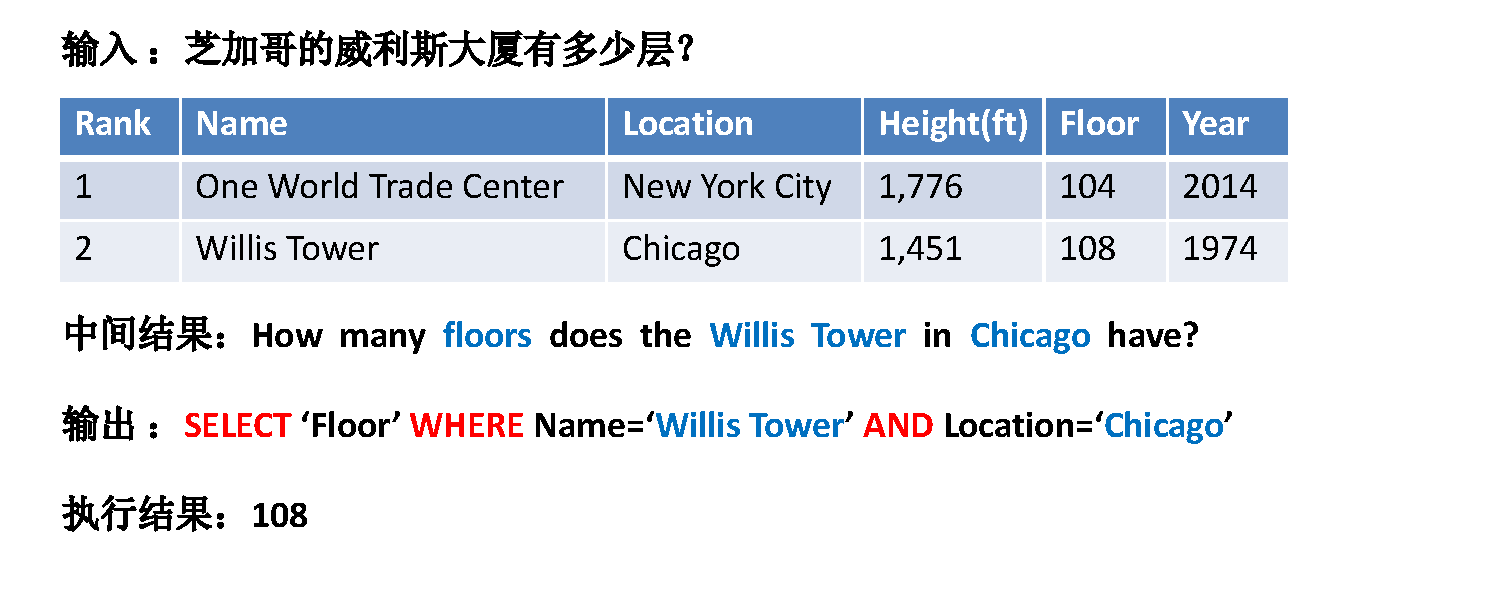
\includegraphics[width=17cm]{example/cnl2sql.pdf}
    \bicaption[这里将出现在插图索引中]
      {中文自然语言问题生成SQL查询语句的示例}
      {English caption}
    \label{fig:cnl2sqlexample}
  \end{figure}

在图\ref{fig:cnl2sqlexample}中,$w$代表中文自然语言问题“芝加哥的威利斯大厦有多少层?”,其中$w_0,w_1,w_2,...$分别代表单词“芝加哥”、“的”、“威利斯大厦”等。
$c$代表数据库表的模式“Name Location Height(ft) Floor Year”,其中$c_0,c_1,c_2,...$分别代表单词“Name”、“Location”、“Height(ft)”等。
总输入$x$代表由$w$和$c$组成的集合。
在将中文的自然语言问题转换为SQL查询语句的过程中会生成中间结果“How  many  floors  does  the  Willis  Tower  in  Chicago  have?”,即将中文翻译为英文,记作$m$。
模型的输出$y$在该示例中对应的SQL查询语句为“SELECT ‘Floor’ WHERE Name=‘Willis Tower’ AND Location=‘Chicago’”,其在数据库中执行的结果$r$为108。

基于多任务学习的NL2SQL生成的主要任务是要在将中文翻译为英文的同时,理解中文自然语言语句的意图并在一次交互的状态下将意图映射到SQL查询语句上,
即在知道数据库表模式$c$的状态下,将用户输入的自然语言问题$w$最终转换为一条SQL查询语句$y$并得到数据库执行结果$r$。

\section{相关技术}
\subsection{注意力转换器模型}

2017年谷歌提出了注意力转换器模型(Transformer)[!!引用!!],其在翻译任务上的表现十分优异。
在该模型中,最重要的机制为多头自注意力机制(multi-head self-attention)和位置编码机制(Positional Encoding)。

\textbf{多头自注意力机制(multi-head self-attention)}

\begin{figure}[!htp]
  \centering
  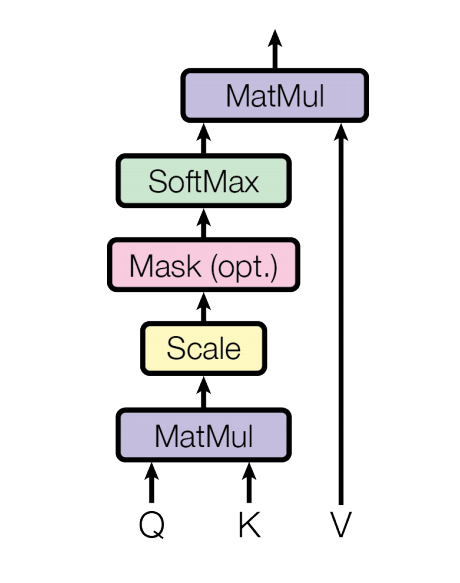
\includegraphics[width=7cm]{example/SDPA.png}
  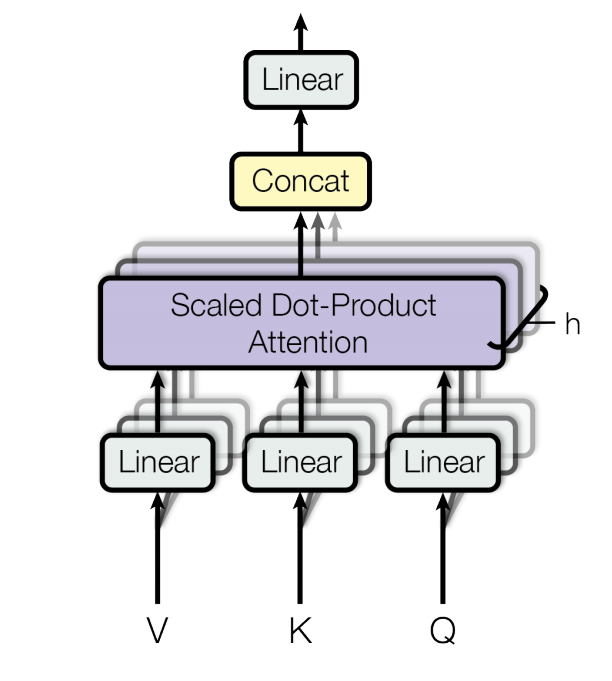
\includegraphics[width=7cm]{example/MHA.png}
  \bicaption[这里将出现在插图索引中]
    {缩放点积注意力(scaled dot-product attention)和多头注意力(multi-head attention)}
    {English caption}
  \label{fig:SDPAMHA}
\end{figure}

多头自注意力机制包含缩放点积注意力(scaled dot-product attention)和多头注意力多头注意力(multi-head attention)两部分,如图\ref{fig:SDPAMHA}所示)。
在缩放点积注意力中,输入由query(Q),$d_k$维的key(K)以及$d_v$维的value(V)组成,需要将query和一些列的(key,value)对映射起来,如公式\ref{cnl2sqleq:mhsaeq1}。
实际上,注意力机制就是一个由诸多Query和(key,value)组成的映射函数。

\begin{equation}
  \label{cnl2sqleq:mhsaeq1}
  q -> [(k_1,v_1),(k_2,v_2),...] -> attention = w_1 * v_1 + w_2 +v_2 + ... 
\end{equation}

query和所有key计算点积,然后除以$\sqrt{d_k}$并计算$softmax$值,得到value对应的权重$w$,如公式\ref{cnl2sqleq:mhsaeq2}。

\begin{equation}
  \label{cnl2sqleq:mhsaeq2}
  Attention(Q,K,V) = softmax(\frac{QK^T}{\sqrt{d_k}})V  
\end{equation}

而多头注意力实际上就是将query和key做多次的线性映射,最后将结果串联在一起。
在编码器和解码器结构中,query来自于上一层的解码器中,而key和value来自上一层的编码器中。
多头注意力就是将句子中的每一个部分都参与到编码和解码的过程中,允许模型关注来自不同位置及不同表示的信息,如公式\ref{cnl2sqleq:mhsaeq3}。

\begin{equation}
  \label{cnl2sqleq:mhsaeq3}
  MultiHead(Q,K,V) = Concat(head_1,...,head_h) \quad \mbox{其中} head_i = Attention(QW^Q_i,KW^K_i,VW^V_i)
\end{equation}

\textbf{位置编码机制(Positional Encoding)}

鉴于注意力转换器模型并没有CNN或RNN的结构,为了引入序列的位置信息,还需要加入位置编码机制。
在编码器和解码器的嵌入之后的向量与$d_{model}$维的位置编码进行求和。
位置编码的方式有很多种,可以是学习得到的也可以是固定的,可以对不同序列使用$sin$和$cos$函数进行计算,如公式\ref{cnl2sqleq:mhsaeq4}。

\begin{gather}
  \label{cnl2sqleq:mhsaeq4}
  PE_{(pos,2i)} = sin(\frac{pos}{10000^{\frac{2i}{d_{model}}}})\\
  PE_{(pos,2i+1)} = cos(\frac{pos}{10000^{\frac{2i}{d_{model}}}}) 
\end{gather}

\subsection{NLP领域的迁移学习}

在自然语言处理(NLP)领域中有很多重要成果都与迁移学习有关。
例如Word2Vec[!!引用!!],skip-thought Vec[!!引用!!]和Glove[!!引用!!]都是先产生预训练好的词向量,再把这些知识“迁移”到其他应用上。
嵌入(embedding)[!!引用!!]、中间表示(intermediate representation)[!!引用!!]和语言模型中的权重[!!引用!!]都可以被迁移到其他类似的架构[!!引用!!]甚至分类任务[!!引用!!]上。
从机器翻译模型上得到的中间表示可以迁移并提升处理问答、情感分析等任务的模型[!!引用!!]。
使用问答数据集训练的模型与使用推理数据集训练的模型可以完成对方的任务[!!引用!!]。
高质量机器翻译模型与低质量机器翻译模型之间也相互支持[!!引用!!]。
这些研究表明,想要同时学习中文自然语言查询转换英文自然语言查询和英文自然语言查询生成SQL查询语句两个任务是可以迁移的。

\subsection{NLP领域的多任务学习}

2011年,Collobert[!!引用!!]首先提出了可以同时处理多个自然语言问题的解决方案,处理的问题包括分块(chunk)、命名实体识别(NER)、词性标注(POS)、语义角色标注(SRE)等。
之后Hashimoto[!!引用!!]也提出了可以同时处理依赖解析、语义相关和自然语言推理任务的网络结构。
使用跨语种的预料进行机器翻译模型训练时发现,采用多任务学习的方法[!!引用!!]甚至可以一定程度解决零样本的问题。
基于序列到序列的模型采用不同数量的编码器和解码器时[!!引用!!]甚至可以同时学习翻译、解析和图像字幕生成的任务。
甚至学习图像分类和语音识别任务的模型可以被模块化[!!引用!!]之后拓展到图像到文字的问答任务上[!!引用!!]。
采用[!!引用!!]的方法还可以减轻任务之间存在的干扰。

事实上,1997年Caruana[!!引用!!]就证明多任务学习是有效的,因为模型能够利用任务之间的关联性。
当同时学习的任务十分相关时,学习不同的任务可以提供归纳偏差[!!引用!!],强迫模型去学习那些更通用和普遍的表示方法。
通过将许多单独的任务同时学习并比较,可以充分验证多任务学习的有效性[!!引用!!]。

显然,本文使用TCR模板将子任务转换为统一形式后,采用多任务学习的学习策略可以有效地提升模型的性能。

% \subsection{NLP领域的元学习}


\section{解决方案}

在本节中,我们会介绍如何把中文自然语言翻译为英文自然语言任务与英文自然语言生成SQL查询语句任务进行统一,之后提出一种基于多任务学习的神经网络结构并解释说明为何这样的网络结构可以有效地解决中文自然语言问题生成SQL查询语句问题。

\subsection{TCR模板}

首先,中文自然语言问题生成SQL查询语句可以被划分为两个子任务:中文自然语言翻译为英文自然语言任务和英文自然语言问题生成SQL查询语句任务。
在第\ref{chap:enl2sql}章中,本文提出的基于深度强化学习的解决方案已经可以有效的解决NL2SQL问题,并且在WikiSQL数据集和spider数据集上有优异的表现。
所以,我们会有一个非常自然的想法,就是直接使用翻译工具或翻译软件将中文的自然语言问题直接转换为英文自然语言问题,之后再使用\ref{enl2sql:zqjxqmx}节中提出的增强解析器模型将英文自然语言转换为SQL查询语句。
但是,这种方法会遇到许多问题,如图\ref{fig:cnl2sqlproblem}所示(其中中文自然语言均使用谷歌翻译自动翻译为英文自然语言):

\begin{figure}[!htp]
    \centering
    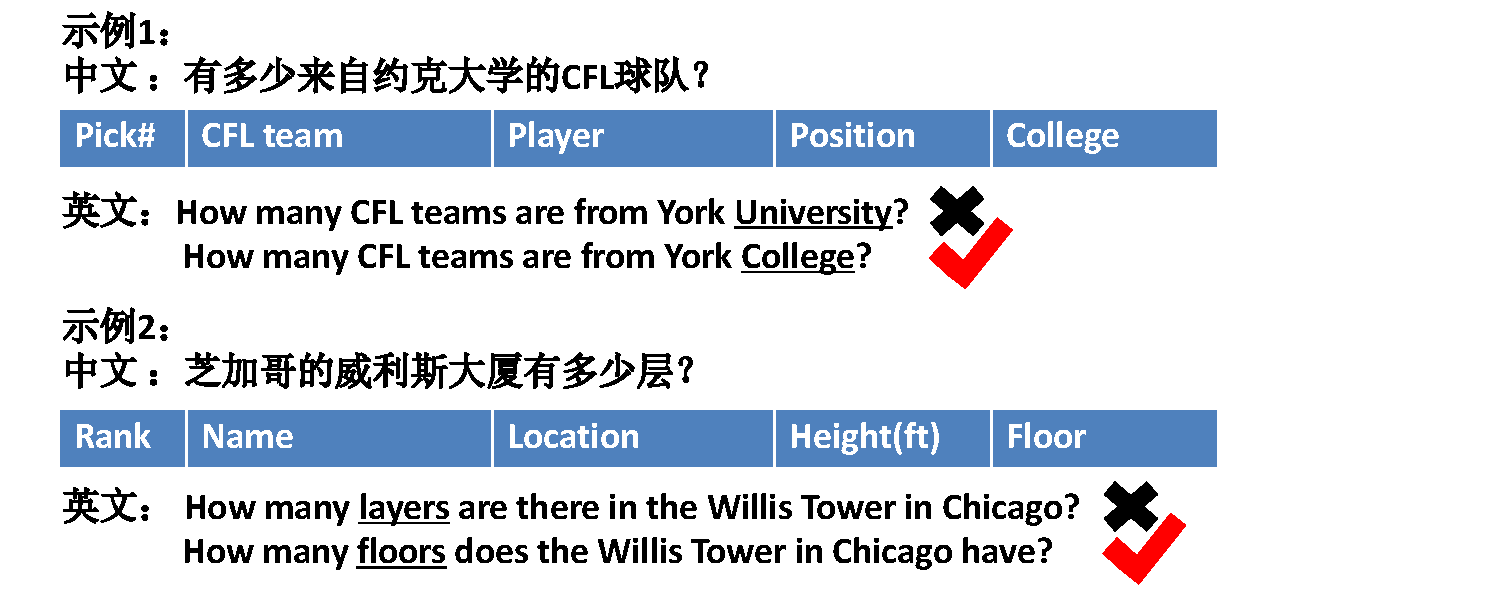
\includegraphics[width=17cm]{example/cnl2sqlproblem.pdf}
    \bicaption[这里将出现在插图索引中]
      {中文自然语言问题生成SQL查询语句的错误示例}
      {English caption}
    \label{fig:cnl2sqlproblem}
  \end{figure}

从图\ref{fig:cnl2sqlproblem}中的示例一可以看出,数据库表模式中的列名为“College”,而谷歌翻译将中文“大学”翻译为“University”。
而示例二中的“层”翻译为了“layers”而不是“floors”。
形如这一类的问题会给SQL的生成带来很大的问题。

究其原因,从中文自然语言到英文自然语言再到SQL查询语句这一过程是一个紧密关联的过程,如果将其拆分为两个部分,则翻译的过程中将会丢失大量的数据库、SQL语言本身的很多信息。
所以,我们提出TCR模板用以将这两个独立的任务有机的统一起来,并在作为下节中的多任务学习网络的输入。

\begin{figure}[!htp]
    \centering
    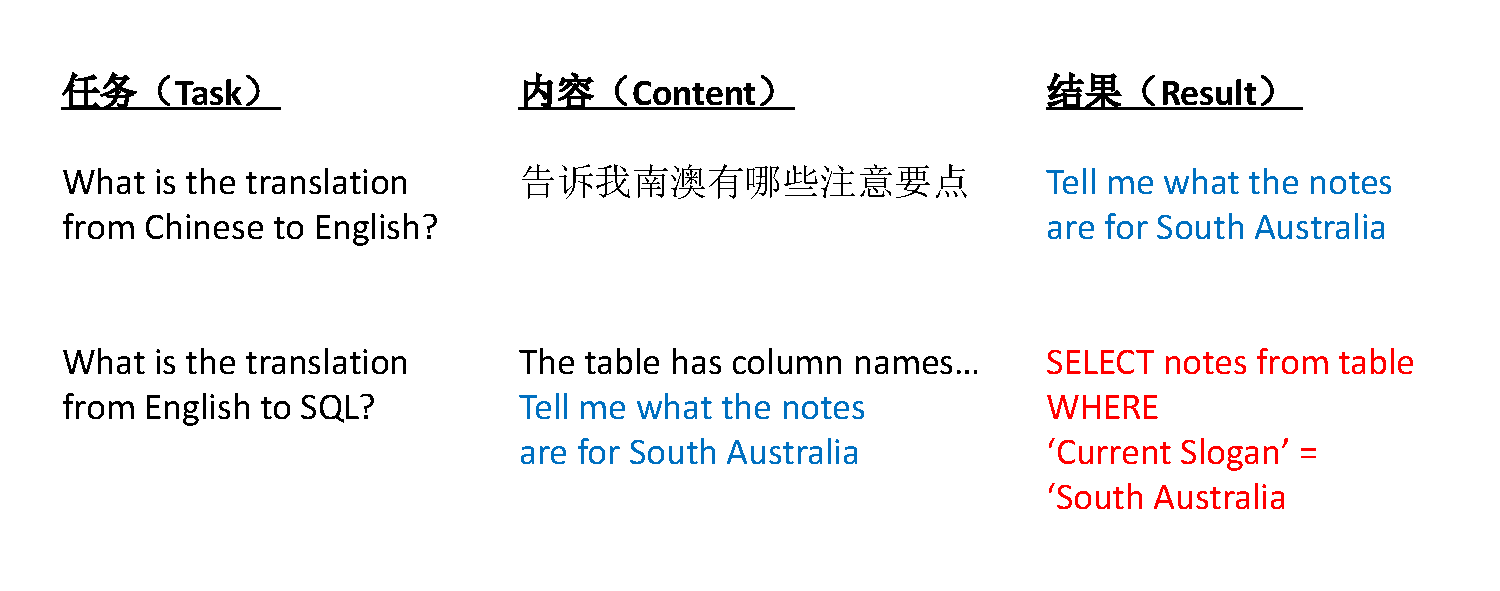
\includegraphics[width=17cm]{example/tcr.pdf}
    \bicaption[这里将出现在插图索引中]
      {TCR模板(任务-内容-结果模板)}
      {English caption}
    \label{fig:cnl2sqltcr}
  \end{figure}

如图\ref{fig:cnl2sqltcr}所示,我们将中文自然语言翻译为英文自然语言任务和英文自然语言生成SQL查询语句任务使用TCR模板(任务-内容-结果)进行统一。
例如,“告诉我南澳有哪些注意要点”先翻译为英文,其任务为“What is the translation from Chinese to English?”(意为需要执行的任务是中文到英文的翻译),内容为“告诉我南澳有哪些注意要点”(指在表明所需要翻译的中文自然语句是什么),结果为“Tell me what the notes are for South Australia”。
而后再将“Tell me what the notes are for South Australia”转换为SQL查询语句,其任务为“What is the translation from English to SQL?”(意为需要执行的任务是英文到SQL的生成),内容为“The table has column names… Tell me what the notes are for South Australia”(指在表明所需的信息由表的列名以及英文自然语言的查询构成),结果为“SELECT notes from table WHERE ‘Current Slogan’ =‘South Australia”,从而完成生成的全过程。

TCR模板将两个任务的模式进行了统一,使得网络模型的输入和输出得以一致,而不用设计两个不同的网络结构来处理这两个任务。
在后文中,我们还将这个模板用于自然语言处理领域中的很多任务,详见\ref{cnl2sql:syyfx}节。

\subsection{多任务网络}

由于我们会使用TCR模板对每个任务进行统一并且在训练阶段采用联合训练的方法,我们把所使用的神经网络的结构称为多任务网络,如图\ref{fig:cnl2sqlnet}所示。
近几年来,有许多研究者所研究的问答模型的和我们的模型比较类似,但是通常的问答模型往往假设模型得到的答案的片段是可以直接从上下文信息中复制,但是我们的多任务网络适用于更一般的问答场景。
在之前的TCR模板中,任务对应于问答模型中的问题,内容对应于问答模型中的上下文,而结果对应于问答模型中的回答。
由于TCR模板中的任务往往包含限制搜索空间的非常关键的信息,我们会在多任务网络中使用了协同注意力机制[!!引用!!]并加以拓展,从而使得对模型输入的表示更加丰富。
此外,多任务网络还采用了指针机制[!!引用!!],并将其改造为分层的多指针生成器,使得网络能够直接从任务和内容中进行文本的复制。

\begin{figure}[!htp]
  \centering
  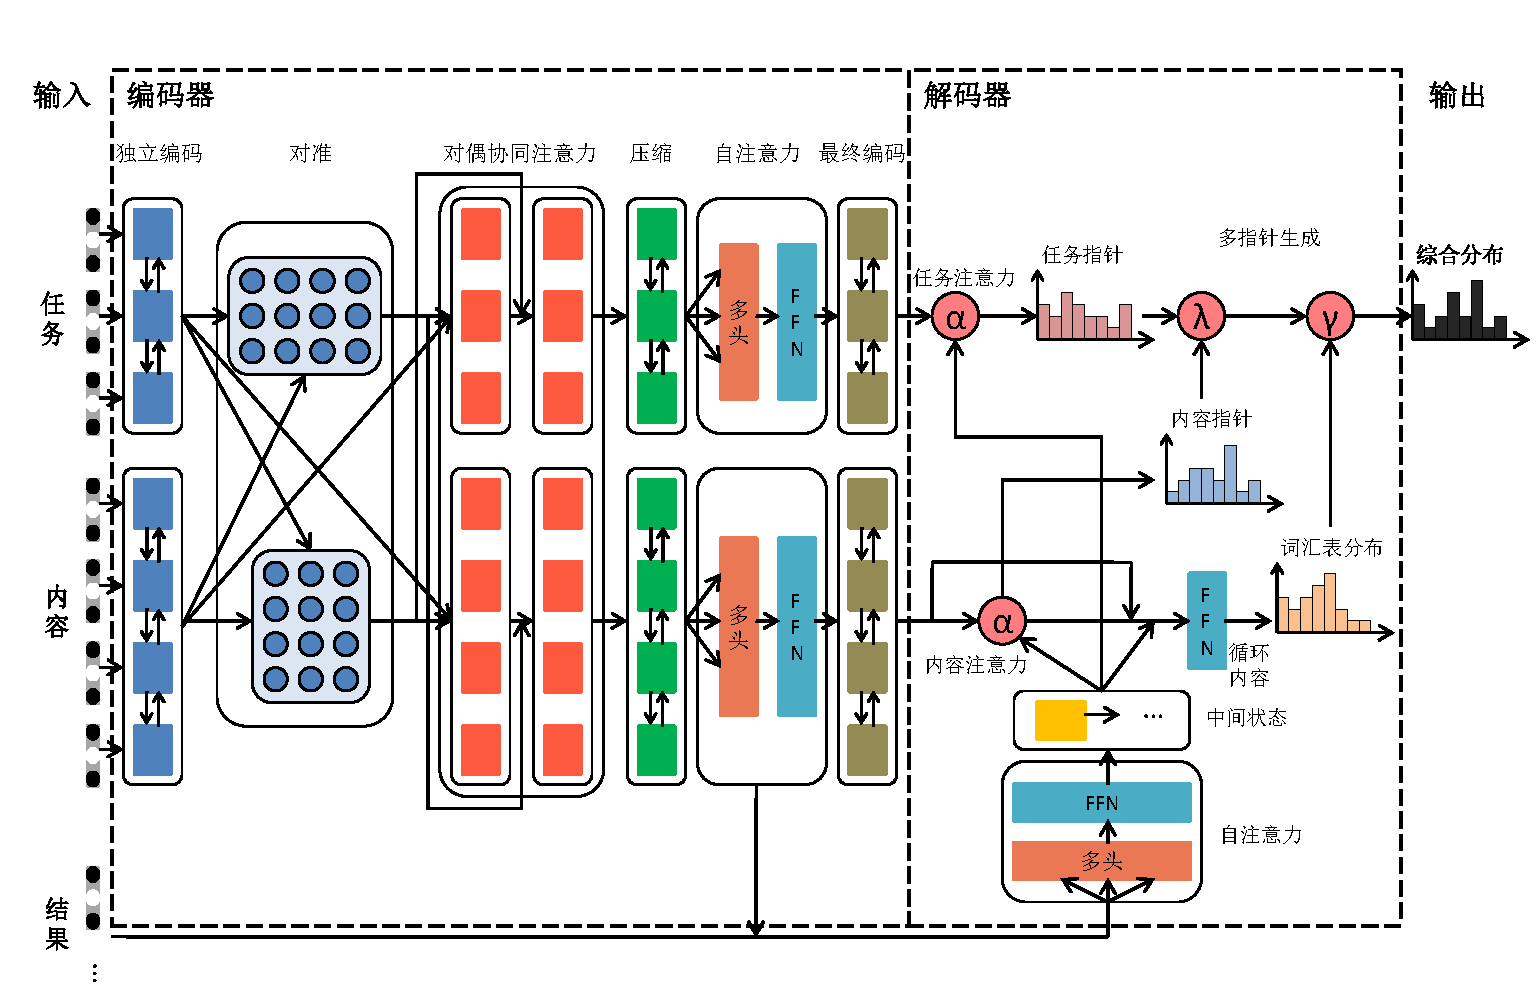
\includegraphics[width=17cm]{example/cnl2sqlnet.pdf}
  \bicaption[这里将出现在插图索引中]
    {多任务网络}
    {English caption}
  \label{fig:cnl2sqlnet}
\end{figure}

在训练阶段,多任务网络的输入序列会有三个部分,分别为:由$l$个单词构成的内容$c$;
由$m$个单词构成的任务$q$;由$n$个单词构成的结果$a$。
其中,每个输入序列都是一个矩阵,矩阵中的第$i$行对应于序列中的第$i$个词的嵌入(embedding)(可为字符向量或词向量),维度为$d_{emb}$。有公式\ref{cnl2sqleq:drwwl1}:
\begin{equation}
    \label{cnl2sqleq:drwwl1}
    C \in \mathbb{R}^{l \times d_{emb}} \qquad Q \in \mathbb{R}^{m \times d_{emb}} \qquad A \in \mathbb{R}^{n \times d_{emb}}
  \end{equation}

接下来,我们将分别详细介绍多任务网络中的编码器和解码器。

\subsection{编码器}
\label{cnl2sql:encoder}

编码器将内容矩阵$C$、任务矩阵$Q$和结果矩阵$A$作为输入,
使用深度栈式循环神经网络[!!引用!!],结合协同注意力机制(coattention)[!!引用!!]和自注意力机制(self-attention)[!!引用!!],
来生成编码阶段的最终的表示$C_{fin} \in \mathbb{R}^{l \times d}$和$Q_{fin} \in \mathbb{R}^{m \times d}$(即编码之后的内容信息和任务信息),
并且还可以让网络学习到他们之间的局部和全局的相互依赖关系。
在下文中,我们将对编码器的每个阶段进行进一步的说明。

\textbf{单独编码阶段}

首先使用一个简单的线性层将输入矩阵投射到$d$维的空间上,如公式\ref{cnl2sqleq:encoder1}。
\begin{equation}
    \label{cnl2sqleq:encoder1}
    CW_1 = C_{proj} \in \mathbb{R}^{l \times d} \qquad QW_1 = Q_{proj} \in \mathbb{R}^{m \times d} 
  \end{equation}
这些投射之后的表示将被输入给一个共享的双向长短期记忆网络(bi-LSTM)[!!引用!!][注释],如公式\ref{cnl2sqleq:encoder2}。
\begin{equation}
    \label{cnl2sqleq:encoder2}
    BILSTM_{ind}(C_{proj}) = C_{ind} \in \mathbb{R}^{l \times d} \qquad BILSTM_{ind}(Q_{proj}) = Q_{ind} \in \mathbb{R}^{l \times d}
\end{equation}

\textbf{对准阶段}

在获得协同注意力的表达之前,我们需要先对每个序列的编码表达进行对准。
我们会分别给$C_{ind}$和$Q_{ind}$增加一个预训练的嵌入使得现在的$C_{ind} \in \mathbb{R}^{(l+1) \times d}$以及$Q_{ind} \in \mathbb{R}^{(m+1) \times d}$,
这样做可以让每个单词不会和序列中的某个单词强制对准。

令$softmax(X)$表示逐列进行softmax操作,即矩阵$X$中的每列进行标准化后的和为1。
我们将内容信息的序列表示与任务序列表示之间进行点积计算得到相似性得分,并使用归一化操作来获得数据的对准,如公式\ref{cnl2sqleq:encoder3}:
\begin{equation}
  \label{cnl2sqleq:encoder3}
  softmax(C_{ind}Q_{ind}^{\top}) = S_{cq} \in \mathbb{R}^{(l+1) \times (m+1)} \qquad softmax(Q_{ind}C_{ind}^{\top}) = S_{qc} \in \mathbb{R}^{(m+1) \times (l+1)}
\end{equation}

\textbf{对偶协同注意力阶段}

再对准之后,我们要去计算一个序列中的某个单词和另一个序列中相关的单词的加权求和,如公式\ref{cnl2sqleq:encoder4}。
\begin{equation}
  \label{cnl2sqleq:encoder4}
  S_{cq}^{\top}C_{ind} = C_{sum} \in \mathbb{R}^{(m+1) \times d} \qquad S_{qc}^{\top}Q_{ind} = Q_{sum} \in \mathbb{R}^{(l+1) \times d}
\end{equation}

对偶协同注意力就是要通过同样的权重将对准时得到的信息传递给原序列,如公式\ref{cnl2sqleq:encoder5}。
\begin{equation}
  \label{cnl2sqleq:encoder5}
  S_{qc}^{\top}C_{sum} = C_{coa} \in \mathbb{R}^{(l+1) \times d} \qquad S_{cq}^{\top}Q_{sum} = Q_{coa} \in \mathbb{R}^{(m+1) \times d}
\end{equation}

可以发现,进行了加权求和和协同注意力的表示中的第一列为之前我们添加进去的冗余的嵌入。
在这里我们不再需要这一个嵌入,所以将矩阵中的这一列去除掉,得到$C_{coa} \in \mathbb{R}^{l \times d}$和$Q_{coa} \in \mathbb{R}^{m \times d}$。

\textbf{压缩阶段}

为了将对偶协同注意力操作之前的信息压缩至$d$维,我们接着把之前得到的四种序列表示进行拼接并输入一个单独的双向LSTM中,如公式\ref{cnl2sqleq:encoder6}。
\begin{align}
  \label{cnl2sqleq:encoder6}
  BiLSTM_{comC}([C_{proj};C_{ind};Q_{sum};C_{coa}]) =  C_{com} \in \mathbb{R}^{m \times d}\\
  BiLSTM_{comQ}([Q_{proj};Q_{ind};C_{sum};Q_{coa}]) =  Q_{com} \in \mathbb{R}^{m \times d}
\end{align}

\textbf{自注意力阶段}

接着,我们使用一个多头的放缩点积注意力机制(multi-head, scaled dot-product attention)[!!引用!!]来捕获每个序列内部的长距离的依赖性,其表达式为公式\ref{cnl2sqleq:encoder7}。

\begin{gather}
  \label{cnl2sqleq:encoder7}
  Attention(\widetilde{X},\widetilde{Y},\widetilde{Z}) = softmax\{\frac{\widetilde{X}\widetilde{Y}^{\top}}{\sqrt{d}}\} \widetilde{Z}\\
  MultiHead(\widetilde{X},\widetilde{Y},\widetilde{Z}) = [h_1;\cdots;h_p]W^o \qquad \mbox{其中}h_j= Attention(\widetilde{X}W^{\widetilde{X}}_j,\widetilde{Y}W^{\widetilde{Y}}_j,\widetilde{Z}W^{\widetilde{Z}}_j)
\end{gather}

公式\ref{cnl2sqleq:encoder7}中变换都为线性变换,所以多头注意力机制可以维持$d$维不变,有公式\ref{cnl2sqleq:encoder8}:
\begin{equation}
  \label{cnl2sqleq:encoder8}
  MultiHead_C(C_{com},C_{com},C_{com}) = C_{mha} \qquad MultiHead_Q(Q_{com},Q_{com},Q_{com}) = Q_{mha}
 \end{equation}

之后,我们使用了一个残差前馈网络(feedforward networks,简称FFN)如公式\ref{cnl2sqleq:encoder9},其中$U \in \mathbb{R}^{d \times f}$,$V \in \mathbb{R}^{f \times d}$。其激活函数为Relu函数[!!引用!!],并且在输入和输出都使用了正则化(layer normalization)[!!引用!!]。
\begin{gather}
  \label{cnl2sqleq:encoder9}
  FFN(X) = \max(0,XU)V + X\\
  FFN_C(C_{com} + C_{mha}) = C_{self} \in \mathbb{R}^{l \times d} \qquad FFN_Q(Q_{com} + Q_{mha}) = Q_{self} \in \mathbb{R}^{m \times d}
\end{gather}

\textbf{最终编码阶段}

最后,我们使用两个双向LSTM将所有信息进行汇总并将矩阵$C_{fin}$和$Q_{fin}$输入给解码器,如公式\ref{cnl2sqleq:encoder10}。
\begin{equation}
  \label{cnl2sqleq:encoder10}
  BiLSTM_{finC}(C_{self}) = C_{fin} \in \mathbb{R}^{l \times d} \qquad BiLSTM_{finQ}(Q_{self}) = Q_{fin} \in \mathbb{R}^{m \times d} 
\end{equation}


\subsection{解码器}
\label{cnl2sql:decoder}

在编码器得到最终的表示$C_{fin} \in \mathbb{R}^{l \times d}$和$Q_{fin} \in \mathbb{R}^{m \times d}$(即编码之后的内容信息和任务信息)后进入到解码器解码。
在下文中,我们将对解码器的每个阶段进行进一步的说明。

\textbf{结果表示阶段}

在训练阶段,解码器首先要将结果$a$的表示投射到$d$维的空间上,如公式\ref{cnl2sqleq:decoder1}

\begin{equation}
  \label{cnl2sqleq:decoder1}
  AW_2 = A_{proj} \in \mathbb{R}^{n \times d} 
\end{equation}

之后紧接的是一个自注意力层,该注意力层与编码器中的自注意力层相对应。
由于该过程不包含循环和卷积操作,所以我们为$A_{proj}$加上了一个位置编码信息$x$,如公式\ref{cnl2sqleq:decoder2}。
\begin{equation}
  \label{cnl2sqleq:decoder2}
  A_{proj} + PE = A_{ppr} \in \mathbb{R}^{n \times d},\qquad \mbox{其中} PE[t,k] = \{   
  \begin{array}{lr}
    sin(\frac{t}{10000^{\frac{k}{2d}}}) &  k\mbox{为偶数}\\
    cos(\frac{t}{10000^{\frac{k-1}{2d}}}) &  k\mbox{为奇数}
  \end{array}
\end{equation}

\textbf{自注意力阶段}
接着我们使用了自注意力机制[!!引用!!]从而使得解码器能够知道之前的输出(若之前没有输出则认为之前的输出为某个初始化的单词)和相关内容是什么,从而产生下一个输出。
在多头的注意力机制之后使用了一个残差前馈网络(FFN,其定义在\ref{cnl2sql:encoder}节中的自注意力阶段给出),如公式\ref{cnl2sqleq:decoder3}。

\begin{gather}
  \label{cnl2sqleq:decoder3}
  MultiHead_A(A_{ppr},A_{ppr},A_{ppr}) = A_{mha} \in \mathbb{R}^{n \times d}\\
  MultiHead_{A}C((A_{mha} + A_{ppr}),C_{fin},C_{fin}) = A_{ac} \in \mathbb{R}^{n \times d}\\
  FFN_A(A_{ac} + A_{mha} + A_{ppr}) = A_{self} \in \mathbb{R}^{n \times d}
\end{gather}

\textbf{获得中间状态阶段}

之后,我们使用了一个标准的带注意力机制的LSTM网络来对每个时刻$t$产生一个内容状态$\widetilde{c}_t$。
这个LSTM又将使用之前的结果序列中的单词$A^{t-1}_{self}$和内容状态来生成一个中间状态$h_t$,如公式\ref{cnl2sqleq:decoder4}。

\begin{equation}
  \label{cnl2sqleq:decoder4}
  LSTM([(A_{self})_{t-1};\widetilde{c}_{t-1}],h_{t-1})= h_t \in \mathbb{R}^{d} 
\end{equation}

\textbf{任务与内容注意力阶段}

上一阶段中的中间状态可用来获得注意力权重$\alpha^C_t$以及$\alpha^Q_t$Q,解码器从而可以获得$t$时刻的编码信息,如公式\ref{cnl2sqleq:decoder5}。

\begin{equation}
  \label{cnl2sqleq:decoder5}
  softmax(C_{fin}(W_2 h_t)) = \alpha^C_t \in \mathbb{R}^{l} \qquad softmax(Q_{fin}(W_3 h_t)) = \alpha^Q_t \in \mathbb{R}^{m}
\end{equation}

\textbf{获得内容与任务状态阶段}

内容的表示将于这些权重相结合并输入给一个前馈网络从而形成内容状态与任务状态,激活函数为$tanh$,如公式\ref{cnl2sqleq:decoder6}。
\begin{equation}
  \label{cnl2sqleq:decoder6}
  tanh(W_4[C^{\top}_{fin}\alpha^C_t;h_t] = \widetilde{c}_{t} \in \mathbb{R}^{d} \qquad tanh(W_5[Q^{\top}_{fin}\alpha^Q_t;h_t] = \widetilde{q}_{t} \in \mathbb{R}^{d}
\end{equation}

\textbf{多指针生成阶段}

由于我们的模型必须要能够生成那些未出现在任务或内容序列中的单词,所以需要额外声明一个词汇表$v$。
我们会从任务、内容和外部的词汇表中分别获得每个单词的概率分布,如公式\ref{cnl2sqleq:decoder7}。

\begin{gather}
  \label{cnl2sqleq:decoder7}
  \sum_{i:c_i=w_t} (\alpha^C_t)_i = p_c(w_t) \in \mathbb{R}^{n}\\
  \sum_{i:q_i=w_t} (\alpha^Q_t)_i = p_q(w_t) \in \mathbb{R}^{m}\\
  softmax(W_v\widetilde{c}_t) = p_v(w_t) \in \mathbb{R}^{v}
\end{gather}

这些概率分布将会覆盖任务、内容和外部词汇表中所有单词的集合,其中却是的一些条目将会被赋为0值从而使所有分布都在$\mathbb{R}^{l+m+v}$。
最后,我们设置两个标量开关来调节每个分布的重要程度并确认最终输出的分布,如公式\ref{cnl2sqleq:decoder8}。
\begin{gather}
  \label{cnl2sqleq:decoder8}
  \sigma (W_{pv}[\widetilde{c}_t;h_t;(A_{self})_{t-1}]) = \gamma \in [0,1]\\
  \sigma (W_{cq}[\widetilde{q}_t;h_t;(A_{self})_{t-1}]) = \lambda \in [0,1]\\
  \gamma p_v(w_t) + (1 - \gamma)[\lambda p_c(w_t) + (1 - \lambda)p_q(w_t)] = p(w_t) \in \mathbb{R}^{l+m+v}
\end{gather}

需要说明的是,在训练的全时域中,我们采用的是单词级别的对数似然损失,如公式\ref{cnl2sqleq:decoder9}。

\begin{equation}
  \label{cnl2sqleq:decoder9}
  \mathcal L = -\sum^T_t \log p(a_t)
\end{equation}


\section{实验与分析}
\label{cnl2sql:syyfx}
\subsection{多任务网络的实验结果}

\begin{table}[!htpb]
  \bicaption[出现在表目录的标题]
    {多任务网络的实验结果}
    {A Table with footnotes}
  \label{tab:drwwldsyjg}
  \centering
  \begin{threeparttable}[b]
     \begin{tabular}{cccccccccc}
      \toprule
      \multirow{2}{18mm}{数据集}&\multicolumn{4}{c}{单任务} & \multicolumn{5}{c}{多任务}\\
      \cmidrule(lr){2-5}\cmidrule(lr){6-10}
      & S2S & w/SAtt & +CAtt & +QPtr & S2S & w/SAtt & +CAtt & +QPtr & +ACurr\\
      \midrule
      % 增强解析器(静态预言) & 87.1 & 88.2 & 65.9 & 67.5\\
      % 增强解析器(非确定性预言, 不解决过滤条件顺序问题) & 88.1 & 89.2 & 68.3 & 69.1\\
      SQuAD & 48.2 & 68.2 & 74.6 & 75.5 & 47.5 & 66.8 & 71.8 & 70.8 & 74.3\\
      IWSLT & 25.0 & 23.3 & 26.0 & 25.5 & 14.2 & 13.6 & 9.0 & 16.1 & 13.7\\
      CNN/DM & 19.0 & 20.0 & 25.1 & 24.0 & 25.7 & 14.0 & 15.7 & 23.9 & 24.6\\
      MNLI & 67.5 & 68.5 & 34.7 & 72.8 & 60.9 & 69.0 & 70.4 & 70.5 & 69.2\\
      SST & 86.4 & 86.8 & 86.2 & 88.1 & 85.9 & 84.7 & 86.5 & 86.2 & 86.4\\
      QA-SRL & 63.5 & 67.8 & 74.8 & 75.2 & 68.7 & 75.1 & 76.1 & 75.8 & 77.6\\
      QA-ZRE & 20.0 & 19.9 & 16.6 & 15.6 & 28.5 & 31.7 & 28.5 & 28.0 & 34.7\\
      WOZ & 85.3 & 86.0 & 86.5 & 84.4 & 84.0 & 82.8 & 75.1 & 80.6 & 84.1\\
      WikiSQL & 60.0 & 72.4 & 72.3 & 72.6 & 45.8 & 64.8 & 62.9 & 62.0 & 58.7\\
      MWSC & 43.9 & 46.3 & 40.4 & 52.4 & 52.4 & 43.9 & 37.8 & 48.8 & 48.4\\
      \midrule
      总得分 & - & - & - & - & 473.6 & 546.4 & 533.8 & 562.7 & 571.7\\
      \bottomrule
    \end{tabular}
  \end{threeparttable}
\end{table}

如图\ref{fig:cnl2sqlnet}以及\ref{fig:cnl2sqltcr}所示,我们的模型的训练样本为包含任务序列、内容序列以及结果序列的三元组。
我们所做的对比实验的基准为使用了指针生成器的序列到序列的模型(简称S2S模型)[!!引用!!]。
不一样的是,S2S模型的输入为自然语言问题序列,而多任务网络的输入为任务及内容序列的集合。

实验结果如表\ref{cnl2sql:syyfx}所示,表中S2S代表序列到序列(sequence to sequence)模型,(w/SAtt)代表增加带自注意力机制的S2S模型,
(+CAtt)代表将任务与内容序列拆分为两个输入序列并增加对偶协同注意力机制,(+QPtr)代表增加任务指针器, (+ACurr)代表增加反递进学习过程。
总得分表示多任务学习时各个子任务得分的和,由于单任务不存在多任务的得分和所以标记为’-’。


在表\ref{cnl2sql:syyfx}中的指标可以看出,S2S模型在SQuAD任务上的效果较差,在WikiSQL数据集上的得分比之前的序列到序列的基准方案要高,但是普遍都没有多任务网络(+QPtr)的效果优异。
在S2S模型的基础上增加了带自注意力机制层(w/SAtt)的编码器和解码器之后[!!引用!!],模型具备了整合来自任务和内容信息的能力。
从表中可以看出,新的模型在SQuAD任务上提升了20 nF1,QA-SRL任务上提升了4 nF1,WikiSQL上提升了12 LFEM。
模型在WikiSQL上的表现接近了最高水平的范围,在没有使用结构化的方法[!!引用!!]下达到了72.4\%。

接着,我们尝试将任务和内容从输入中进行拆分并增加了对偶协同注意力机制(+CAtt)。
可以看到,模型在SQuAD和QA-SRL上的性能提升了超过5 nF1,但是在其他任务上没有明显的提升,甚至在MNLI和MWSC任务上的性能有所降低。
其原因是由于两个任务往往能够从输入中直接复制一些单词作为输出,S2S模型的输入为任务和内容信息的集合,所以其中的指针生成器可以直接完成从输入中复制信息到输出的操作。
而将任务和内容信息拆分为两个输入序列的时候,模型就失去了这个能力。

为了解决这个问题,我们在之前的模型上又增加了一个任务指针(+QPtr)进行实验。
实验结果显示,任务指针有效的提高了模型在MNLI和MWSC上的性能。
同时,模型在SQuAD任务上提升到了75.5 nF1,达到了SQuAD领域中使用直接跨度检测方法的水平,也就是说多任务网络达到了不明确将问题进行跨度检测的方法中的最高水平。

最后的模型在WikiSQL任务上达到了72.4\%的lfEM以及80.4\%的数据库执行准确率,超过了之前的最高水平[!!引用!!]的71.7\%和78.5\%。

在单任务与多任务的比较中,我们也得到了类似的结果以及注意到了一些额外的特点。
多任务与单任务模型相比,在QA-ZRE任务上的F1得分又有11点提升,也验证了多任务的模型在解决零样本学习(zero-shot learning)上的能力。

\subsection{不同优化策略下的实验结果}

在多任务的训练过程中我们尝试了各种批量采样(batch-level sampling)的策略,包括联合训练、递进学习、反递进学习等,其实验结果如表\ref{tab:drwwlzbtxlclxdsyjg}所示。

我们首先考虑的是完全联合(fully joint)的策略。
从训练开始到结束,我们对所有的任务按照固定的顺序循环的进行批量采样。
这种策略在迭代(iteration)次数较少的单任务下的表现良好,见表\ref{tab:drwwlzbtxlclxdsyjg},但在迭代次数较多的单任务下性能不佳。
经过总结我们发现,单任务与多任务场景下的性能的差异与单任务的迭代次数之间有很强的关联。

由于上述原因,我们还尝试了一些反递进学习的策略[!!引用!!]。
这些训练的策略都是由两阶段组成的:1)在第一阶段中对部分任务进行联合训练(往往选择较难的任务)。2)第二阶段根据完全联合策略进行对所有任务进行训练。

首先,我们尝试了先将SQuAD任务进行单独训练,之后再对其他的所有任务进行完全联合训练。
由于我们的多任务网络对于所有任务来说是一种基于问答的方法,所以我们联想到是否可以先与训练SQuAD这样的QA数据集然后再对其他的类QA的任务进行训练。
这种方法可以使得解码器先学会如何从内容信息中检索出有用信息,然后学习不同的任务以及如何产生属于不同任务领域的单词。
在SQuAD这个任务场景下进行预训练已经被证明可以提高NLI的性能[!!引用!!]。
根据我们的实验来看,这种方式相对于其他的训练策略而言是一种更有效的训练策略,在总得分上获得了571.7的最高分。
需要特别提到的是,这种策略在IWSLT任务上的得分较低,但是在其他的任务中会有更大的提升,特别是使用指针的任务。

为了探索在递进学习策略的初始状态下增加额外的任务是否会进一步提高性能,我们还尝试了将IWSLT、CNN/DM任务和IWSLT、CNN/DM、MNLI任务加入到第一阶段进行训练。
这些任务包含了与其他任务非常相关的训练样本,并且也包含了最长的结果序列。
除此之外,这些任务具有很高的多样性,应该能够让解码器学会更多的解码方式,例如针对IWSLT的词汇表、针对SQuAD与CNN/DM的内容指针以及针对MNLI的任务指针。
然而,实验结果表明这些新增的任务并没有提升模型的性能。
在将SQuAD, IWSLT, CNN/DM和MNLI加入到递进学习的初始状态下时,其他的一些任务(例如QA-SRL, WikiSQL和MWSC)的性能明显下降。

另外,我们也尝试了在递进学习策略的初始状态下使用了SST, QA-SRL, QA-ZRE, WOZ, WikiSQL和MWSC,这也就意味着先选择一些最简单的任务并进行训练。
实验证明,这个策略是一个非常低劣的策略,不仅在初始递进学习中的任务的性能很差,在SQuAD和IWSLT上的表现更差。

事实证明,对于我们的任务而言,使用反递进学习策略的效果优于递进学习策略,也就是说明了先学习简易的任务未能使模型学到能应用于其他任务的表示,甚至使得模型想要学习到其他任务有用的内部表示变得更加地困难。
除此之外,实验的结果也说明了多任务学习的挑战。
通过改变所学习的任务的先后次序可能可以提高某些任务性能,但也很有可能使其他的任务的性能下降。
这也是多任务学习中一个非常值得研究的任务。


\begin{table}[!htpb]
  \bicaption[出现在表目录的标题]
    {多任务网络在不同训练策略下的实验结果}
    {A Table with footnotes}
  \label{tab:drwwlzbtxlclxdsyjg}
  \centering
  \begin{threeparttable}[b]
     \begin{tabular}{cccccc}
      \toprule
      \multirow{2}{18mm}{数据集}&\multirow{2}{18mm}{完全联合}&\multirow{2}{18mm}{递进} & \multicolumn{3}{c}{反递进}\\
      \cmidrule(lr){4-6}
      % & S2S & w/SAtt & +CAtt & +QPtr & S2S & w/SAtt & +CAtt & +QPtr & +ACurr\\
      & & & SQuAD & +IWSLT+CNN/DM & +MNLI\\
      \midrule
      SQuAD & 70.8 & 43.4 & 74.3 & 74.5 & 74.6\\
      IWSLT & 16.1 & 4.3 & 13.7 & 18.7 & 19.0\\
      CNN/DM & 23.9 & 21.3 & 24.6 & 20.8 & 21.6\\
      MNLI & 70.5 & 58.9 & 69.2 & 69.6 & 72.7\\
      SST & 86.2 & 84.5 & 86.4 & 83.6 & 86.8\\
      QA-SRL & 75.8 & 70.6 & 77.6 & 77.5 & 75.1\\
      QA-ZRE & 28.0 & 24.6 & 34.7 & 30.1 & 37.7\\
      WOZ & 80.6 & 81.9 & 84.1 & 81.7 & 85.6\\
      WikiSQL & 62.0 & 68.6 & 58.7 & 54.8 & 42.6\\
      MWSC & 48.8 & 41.5 & 48.4 & 34.9 & 41.5\\
      \midrule
      % 总得分 & - & - & - & - & 473.6 & 546.4 & 533.8 & 562.7 & 571.7\\
      总得分 & 562.7 & 499.6 & 571.7 & 546.2 & 557.2\\
      \bottomrule
    \end{tabular}
  \end{threeparttable}
\end{table}

\subsection{实验分析}

\textbf{多指针生成器与任务识别}

多任务网络会从三个方面进行选择:从词汇表生成词汇、任务序列上的指针以及内容序列上的指针。
尽管模型没有明确的监督信号来训练这些选择,但网络仍可以学会如何在这三个选择之间进行切换。
图xx显示了我们最好的模型选择每个选项的频率是怎样的。
可以看出,对于SQuAD,QA-SRL和WikiSQL任务,模型主要是从内容信息中进行选择和复制,这正是因为这些任务中的正确结果主要攘括在内容中。
由于答案的摘要主要由内容中的单词组成,模型在CNN/DM任务中也是主要从内容中进行复制。
对于SST,MNLI和MWSC,由于任务序列中会包含需要的类别,所以模型也偏向选择任务指针。
对于IWSLT和WOZ,模型更喜欢选择从词汇表生成单词,因为中文的单词和对话的状态字段很少在对应的内容信息中。

同时,使用了TCR模板之后的所有任务之间不会使得模型产生混淆。例如:中文单词仅仅会在中文翻译成英文的过程中出现,而在情感分析任务中也从未输出过非“正面”或“负面”的情感类别。

\textbf{模型的拓展性}

多任务网络具有很好的拓展性,除了中文翻译为英文任务和英文生成SQL自然语言任务外对图\ref{cnl2sql:syyfx}中的其他任务都有很好的表现。
在这十个任务共同学习的模型的基础上进行其他任务的学习更加表现了模型良好的拓展性。
对于两个新的任务,英文到捷克语的翻译任务以及命名实体识别(NER)上,使用训练好的模型进行微调可以在更少的迭代次数下达到模型的收敛,达到很好的效果,如图xx。
其中,英文到捷克语的翻译任务使用的是En->Cs数据集,NER任务使用的是OntoNotes 5.0数据集[!!引用!!]。

\textbf{文本分类的零样本学习}

由于MNLI包含在是个任务中,因此模型也可以适应斯坦福自然语言推理语料库(SNLI)[!!引用!!]。
在预训练的多任务网络之上进行微调可以达到87%的精确匹配分数,比随机初始化再训练提升了2分,也比现有的最高水平提升了了2分[!!引用!!]。
更值得注意的是,在没有对SNLI进行任何微调的情况下,在原模型上预训练的多任务网络仍然达到了62%的精确匹配分数。
因为十个任务包含SST任务,所以它也可以在其他二元情感分类任务上表现良好。 
在亚马逊和Yelp评论数据集[!!引用!!]上,预训练的多任务网络分别达到了82.1\%和80.8\%的精确匹配分数并且不需要对模型进行任何微调。
这些结果表明在多任务网络模型的基础上进行微调可以是的模型拓展到域外的问题上,甚至可以适应更广的文本分类问题上。

\section{本章小结}

%# -*- coding: utf-8-unix -*-
% !TEX program = xelatex
% !TEX root = ../thesis.tex
% !TEX encoding = UTF-8 Unicode
%%==================================================
%% conclusion.tex for SJTUThesis
%% Encoding: UTF-8
%%==================================================
\chapter{总结与展望}
\label{chap:conculution}
\section{本文贡献}

随着IT和互联网技术的发展,关系型数据库和数据库技术被广泛地使用并作为数据存储的主要方式。
越来越多的软件技术人员和业务人员需要使用SQL查询语句从数据库中获得所需的信息。
然而,掌握SQL语言需要使用者经过数据库和SQL相关知识的培训,且在使用时需要确切了解数据库的模式等信息。
如果可以让使用者通过交互式的自然语言接口甚至直接使用自然语言来对数据库执行查询将大大缩短业务与技术的鸿沟,极大地提升软件的生产效率。
在此背景下,本文对SQL查询语句的生成技术进行了研究,提出了基于映射的INL2SQL生成、基于深度强化学习的NL2SQL生成和基于多任务学习的NL2SQL生成三种解决方案。

本文的主要贡献和创新点包括:

\textbf{1)交互式自然语言接口生成SQL查询语句的方法}

本文提出了交互式自然语言接口生成SQL语句模型的设计和具体实现,基本思想是结合自然语言解析技术,使用人机交互的方式指导解析过程。
通过依赖解析树生成、解析树节点映射、解析树优化重构、查询树翻译模块对用户输入的查询进行意图的解析并映射到SQL查询语句上。
通过交互式对话器和用户接口模块对意图解析和映射进行补充和重构。
减少了自然语言解析中出现的歧义问题和错误情况,提升了准确性。


\textbf{2)英文自然语言生成SQL查询语句的方法}

本文提出了一种基于深度强化学习的NL2SQL生成的解决方案。
在离线训练阶段,将WikiSQL中的数据进行序列表示后输入给网络模型,模型生成SQL查询语句后在数据库中执行,再使用奖励函数构造奖励用于强化网络模型。
在在线生成阶段用户输入自然语言查询语句及数据库模式,训练好的网络模型将生成符合用户查询意图的SQL查询语句。
我们把其中最重要的网络模型称为“增强解析器”模型,它由编码器和解码器构成并结合了自注意力机制。
参考强化学习的基本范式,本文将增强解析器学习的目标转换为策略的优化问题并对给出了解析器的状态和动作的定义。
为了解决SQL查询语句中的过滤条件的顺序问题以及隐式列名的问题,本文还提出了非确定性预言和$ANYCOL$状态的解决办法。
在与目前NL2SQL领域的前沿方法进行对比以及在不同数据集上的实验结果证明了本文方法的有效性与前瞻性。

\textbf{3)中文自然语言生成SQL查询语句的方法}

为了进一步提高NL2SQL生成的准确性以及解决中文自然语言生成SQL查询语句的问题,本文还提出了一种基于多任务学习的NL2SQL生成的解决方案。
为了解决输入一致性的问题,本文首先提出使用TCR模板对中文自然语言转换为英文自然语言任务和英文自然语言转换为SQL查询语句任务进行统一。
再使用由编码器和解码器构成的多任务网络模型。
其中,编码过程包含单独编码、对准、对偶协同注意力、压缩、自注意力和最终编码阶段;
解码过程包含结果表示、自注意力、获得中间状态、任务与内容注意力、获得任务与内容状态、多指针生成阶段。
本文进行了多任务网络的实验、不同优化策略下的实验、应用在更多的任务上的实验结果证明了本文方法不仅能够提升英文自然语言生成SQL查询语句任务的准确性,还能够很好地完成中文自然语言生成SQL语言任务,同时还具有很好地可拓展性。

\section{展望}

由于时间和能力有限,可以在以下几个方面做进一步的研究和改进:

\textbf{1)交互式自然语言接口生成SQL查询语句的泛化能力}

从本文的实验结果可以看出,模型存在无法处理子查询、所需输入的自然语言意图形式较固定、无法处理特殊词组等问题,需要进一步进行提升和改进。
可以考虑使用深度学习进行语义分类、命名实体识别等手段辅助进行意图的提取。
还可以采用将深度学习和模块化的工程相结合的方法,提升系统对于子查询的处理能力。
除此之外,本文的交互方法较为简单,接下来还可以考虑将任务型问答系统的相关技术(例如,槽填充技术)运用在与用户的多轮交互中,从而更好地解决歧义和信息缺失的问题。


\textbf{2)复杂SQL语句的自动生成}

本文及其他最新的研究工作所使用到的数据集都是以WikiSQL数据集为主,而WikiSQL数据属于spider数据集中定义的简单和中等难度。
本文提出的解决方案已经几乎达到简单和中等难度的SQl查询语句生成的最佳性能,之后的模型需要更多地考虑解决语句的多样性和复杂性。
可以通过分析困难和极难难度的SQL查询语句的特性来设计新的更复杂的神经网络结构,可以考虑将深度学习和模块化的工程相结合的办法解决单个神经网络无法解决的问题。
另外,SQL查询语句只是SQL语句中结构最简单、语义最清楚的一种,而范围更大的SQL语句的自动生成任务是更具挑战的。

\textbf{3)中文自然语言生成SQL查询语句}

除了英文自然语言生成SQL查询语句之外,中文自然语言生成SQL查询是更具难度的。
首先,目前还没有从中文自然语言生成SQL查询语句的训练数据集,今后的研究可以先构造出这样的数据集。
同时,由于数据库表模式往往使用的是英文甚至是英文缩写,这也很大程度的提高了这个研究领域的难度。
其次,本文使用了多任务的网络同时学习中英翻译和英文生成SQL两个任务的解决方案,在一定程度上解决了中文生成SQL语句的问题。
但是,随着查询语句变得复杂和冗长、SQL语句格式更长更深的时候,研究者还需要找到两者存在的更多共性从而解决问题。



% \begin{summary}

% 这里是全文总结内容。

% 2015年2月28日,中央在北京召开全国精神文明建设工作表彰暨学雷锋志愿服务大会,公布全国文明城市(区)、文明村镇、文明单位名单。上海交通大学荣获全国文明单位称号。         

% 全国文明单位这一荣誉是对交大人始终高度重视文明文化工作的肯定,是对交大长期以来文明创建工作成绩的褒奖。在学校党委、文明委的领导下,交大坚持将文明创建工作纳入学校建设世界一流大学的工作中,全体师生医护员工群策群力、积极开拓,落实国家和上海市有关文明创建的各项要求,以改革创新、科学发展为主线,以质量提升为目标,聚焦文明创建工作出现的重点和难点,优化文明创建工作机制,传播学校良好形象,提升社会美誉度,显著增强学校软实力。2007至2012年间,上海交大连续三届荣获“上海市文明单位”称号,成为创建全国文明单位的新起点。         

% 上海交大自启动争创全国文明单位工作以来,凝魂聚气、改革创新,积极培育和践行社会主义核心价值观。坚持统筹兼顾、多措并举,将争创全国文明单位与学校各项中心工作紧密结合,着力构建学校文明创建新格局,不断提升师生医护员工文明素养,以“冲击世界一流大学汇聚强大精神动力”为指导思想,以“聚焦改革、多元推进、以评促建、丰富内涵、彰显特色”为工作原则,并由全体校领导群策领衔“党的建设深化、思想教育深入、办学成绩显著、大学文化丰富、校园环境优化、社会责任担当”六大板块共28项重点突破工作,全面展现近年来交大文明创建工作的全貌和成就。         

% 进入新阶段,学校将继续开拓文明创建工作新格局,不断深化工作理念和工作实践,创新工作载体、丰富活动内涵、凸显创建成效,积极服务于学校各项中心工作和改革发展的大局面,在上级党委、文明委的关心下,在学校党委的直接领导下,与时俱进、开拓创新,为深化内涵建设、加快建成世界一流大学、推动国家进步和社会发展而努力奋斗!       

% 上海交通大学医学院附属仁济医院也获得全国文明单位称号。      

% \end{summary}


\appendix % 使用英文字母对附录编号

% % 附录内容,本科学位论文可以用翻译的文献替代。
% \include{tex/app_setup}
% \include{tex/app_eq}
% \include{tex/app_cjk}
% \include{tex/app_log}

\backmatter % 文后无编号部分 

% 参考资料
\printbibliography[heading=bibintoc]

% 致谢、发表论文、申请专利、参与项目、简历
% 用于盲审的论文需隐去致谢、发表论文、申请专利、参与的项目
\makeatletter

% "研究生学位论文送盲审印刷格式的统一要求"
% http://www.gs.sjtu.edu.cn/inform/3/2015/20151120_123928_738.htm

% 盲审删去删去致谢页
\ifsjtu@review\relax\else
  %# -*- coding: utf-8-unix -*-
% !TEX program = xelatex
% !TEX root = ../thesis.tex
% !TEX encoding = UTF-8 Unicode
\begin{thanks}

  % 感谢所有测试和使用交大学位论文 \LaTeX 模板的同学!

  % 感谢那位最先制作出博士学位论文 \LaTeX 模板的交大物理系同学!

  % 感谢William Wang同学对模板移植做出的巨大贡献!
  
  % 感谢 \href{https://github.com/weijianwen}{@weijianwen} 学长一直以来的开发和维护工作!
  
  % 感谢 \href{https://github.com/sjtug}{@sjtug} 以及 \href{https://github.com/dyweb}{@dyweb} 对 0.9.5 之后版本的开发和维护工作!
  
  % 感谢所有为模板贡献过代码的同学们, 以及所有测试和使用模板的各位同学!

一转眼,我的的研究生生涯即将结束了,回想自己在交大的这两年半的时光,感触良多。
在此我要向研究生期间给予过我指导的所有老师、陪伴我成长的各位同学致以诚挚的感谢。

首先,我要对我的研究生导师沈备军老师表示感谢。
在科研方面,沈老师一直鼓励和尊重我选择自己感兴趣的研究方向,引导并指导我的研究内容,
沈老师认真严谨的办事作风和勤勤恳恳的工作态度给我留下了深刻的印象。
在工程开发上,沈老师让我积极地参与和主导实验室的项目,使我积累了一定的项目经验并提高了技术水平。
在生活中,沈老师也非常关心我的身体健康,主动为我排忧解难。
此外,沈老师资助我前往美国参加国际会议,让我开阔了视野并结识了许多优秀的同行。

还要感谢研究生期间所有的老师,他们孜孜不倦的教诲使我丰富了知识,细致入微的工作使我们可以顺利并愉快地度过这两年半的时光。
感谢莫文凯和陈凯学长,在我做研究实验与发表论文时都给予我很大的帮助,为我树立了榜样。
感谢黄卫智、杨宇、李宁和董翔学长,不仅在项目开发上为我解答释疑,在毕业之后还与我分享工作心得与感悟,让我不断成长。
感谢实验室的所有同学,我们一起做项目、一起讨论技术难题、一起团队建设,大家的陪伴与支持让我能够一路前行。

最后,我要感谢我的父母和女友,和你们在一起是我最轻松和快乐的时候。
无论我是否努力,是否优秀,不管我做怎样的决定,你们都一直在我的身后坚定地支持我。

\end{thanks}
         % 致谢
\fi

\ifsjtu@bachelor
  % 学士学位论文要求在最后有一个英文大摘要,单独编页码
  \include{tex/end_english_abstract}
\else
  % 盲审论文中,发表学术论文及参与科研情况等仅以第几作者注明即可,不要出现作者或他人姓名
  \ifsjtu@review\relax
    %# -*- coding: utf-8-unix -*-
% !TEX program = xelatex
% !TEX root = ../thesis.tex
% !TEX encoding = UTF-8 Unicode

\begin{publications}{99}
    \item\textsc{第一作者}. {EI国际会议论文}, 2017.  
    \item\textsc{第一作者}. {SCI国际期刊论文}, 2017.
\end{publications}

    \include{tex/projectsreview}  
  \else
    %# -*- coding: utf-8-unix -*-
% !TEX program = xelatex
% !TEX root = ../thesis.tex
% !TEX encoding = UTF-8 Unicode
%%==================================================
%% pub.tex for SJTUThesis
%% Encoding: UTF-8
%%==================================================

\begin{publications}{99}
    \item\textsc{Xiong Y, Meng Z, Shen B}, et al. {Mining Developer Behavior Across GitHub and StackOverflow}[C] International Conference on Software Engineering and Knowledge Engineering. 2017:578-583.
    % Xiong Y, Meng Z, Shen B Mining Developer Behavior Across GitHub and StackOverflow[C]// The, International Conference on Software Engineering and Knowledge Engineering. 2017:578-583.
% Xiong Y, Meng Z, Shen B Developer Identity Linkage and Behavior Mining Across GitHub and StackOverflow[J]. International Journal of Software Engineering & Knowledge Engineering, 2018, 27(9n10):1409-1425.
    \item\textsc{Xiong Y, Meng Z, Shen B}, et al. {Developer Identity Linkage and Behavior Mining Across GitHub and StackOverflow}[J]. International Journal of Software Engineering \& Knowledge Engineering, 2018, 27(9n10):1409-1425.
    % \item\textsc{Chen H, Chan C~T}. {Acoustic cloaking in three dimensions using acoustic metamaterials}[J]. Applied Physics Letters, 2007, 91:183518.
    % \item\textsc{Chen H, Wu B~I, Zhang B}, et al. {Electromagnetic Wave Interactions with a Metamaterial Cloak}[J]. Physical Review Letters, 2007, 99(6):63903.
\end{publications}
       % 发表论文
    \include{tex/projects}  % 参与的项目
  \fi
\fi

% \include{tex/patents}     % 申请专利
% \include{tex/resume}      % 个人简历

\makeatother

\end{document}
